\sloppy
% =====================================================================
% Appendix for main.tex. Sections carry the labels referenced from the
% main text: app:proofs, app:support, app:lean, app:protocol, app:eeg,
% app:hyper, app:repro.
% =====================================================================

% Compact restatements of main-text results, numbered as in Section 4.
\newenvironment{restated}[1]{%
  \par\medskip\noindent\textbf{#1 (restated).}\hspace{0.4em}\ignorespaces
}{\par\smallskip}

% Remarks (own counter; the shared theorem counter of the main text is
% untouched, so the numbering of Section 4 is preserved).
\newtheorem{remark}{Remark}

% Appendix floats carry their section letter (D.1, E.1, ...).
\renewcommand{\thefigure}{\thesection.\arabic{figure}}
\renewcommand{\thetable}{\thesection.\arabic{table}}

\section{Proofs of Section~\ref{sec:theory}}
\label{app:proofs}

This appendix proves the results of Section~\ref{sec:theory} in full, restating each numbered claim or setting it up in the notation of its proof.
Throughout, $(x_t, y_t)_{t \ge 1}$ is a stream with $x_t \in \R^D$ obeying
$y_t = x_t^\top w^*_t + \varepsilon_t$, where $\mathcal F_t$ is the $\sigma$-algebra generated by the past, $\E[\varepsilon_t \mid \mathcal F_t] = 0$, and $\E[\varepsilon_t^2 \mid \mathcal F_t] \le \sigma^2$.
The learner maintains sufficient statistics
\[
  A_t = \alpha A_{t-1} + x_t x_t^\top, \qquad
  B_t = \alpha B_{t-1} + x_t y_t, \qquad
  n_t = \alpha n_{t-1} + 1,
\]
with forgetting $\alpha \in (0,1]$ and initialization from a warm-up set of $T_w$ samples.
Write $\bar A_t = A_t/n_t$ with eigendecomposition $\bar A_t = U\,\mathrm{diag}(\mu_1,\dots,\mu_D)\,U^\top$ and $\bar b_t = B_t/n_t$; an index $i$ always refers to the coordinate in this eigenbasis.
\emph{Two design models.} Lemma~\ref{lem:zerolag} and Theorems~\ref{thm:cadence}--\ref{thm:window} are proved in the \emph{mean-field} model $\bar A_t \equiv \Sigma$, i.e.\ the random accumulator is replaced by its population expectation; this is the model in which the lag, the variance factor $\Psi$, and the window target are exact. Theorem~\ref{thm:rmt} is the finite-$D$ \emph{random-design} correction: it retains the random $\bar A_t$ and takes the proportional limit $\zeta = D\omega$ fixed. The two agree as $\zeta \to 0$; the grid's pre-drift windows have $\zeta \le 0.13$, while drift-phase windows reach $\zeta \le 6.4$, where the mean-field target is a control law, not the exact optimum (Appendix~\ref{app:proofs}, ``Regime of the first-order variance term'').
The anchored solve with anchor $G_t$ and strength $\rho > 0$ is $W_t = (A_t + n_t\rho I)^{-1}(B_t + n_t\rho G_t)$; in the eigenbasis, coordinate $i$ is the scalar problem
\begin{equation}
\label{eq:app-anchored}
  W_{t,i} \;=\; \frac{\bar b_{t,i} + \rho\,G_{t,i}}{\mu_{t,i} + \rho}
  \;=\; (1 - s_i)\,\widehat w_{t,i} + s_i\,G_{t,i},
  \qquad
  s_i \;=\; \frac{\rho}{\mu_{t,i} + \rho},
\end{equation}
where $\widehat w_{t,i} = \bar b_{t,i}/\mu_{t,i}$ is the per-direction data solution.
Under the warm-up model the data solution is unbiased per direction with variance $v_i = \sigma^2/(n_t \mu_{t,i})$.
Two parametrizations of the anchored family are used: the \emph{scalar-$\rho$} family (one $\rho$; the pull $s_i = \rho/(\mu_i + \rho)$ is then spectrum-adaptive) and the \emph{uniform-$s$} family (one pull $s$ for all directions, i.e.\ $\rho_i = \mu_i s/(1-s)$; the solution path is the segment between $\widehat w$ and $G$).
Both satisfy the pull identity, which underlies every result below.

\subsection{Proof of Equation~\eqref{eq:pull} (pull identity)}
\label{app:proof-pull}

\begin{restated}{Equation (1)}
Let $\mu > 0$, $\rho > 0$, and $b, g, w, \gamma \in \R$.
Define $s = \rho/(\mu + \rho)$, $\widehat w = b/\mu$, and $W = (b + \rho \gamma g)/(\mu + \rho)$.
Then, exactly,
\[
  W - w \;=\; (1 - s)\,(\widehat w - w) \;+\; s\,(\gamma g - w).
\]
In particular, for $\gamma = 1$ the anchored error is a convex combination of the data error and the anchor error, per direction.
\end{restated}

\begin{proof}[Proof of Equation~\eqref{eq:pull}]
Since $1 - s = \mu/(\mu + \rho)$,
\[
  (1 - s)\,\widehat w + s\,\gamma g
  \;=\; \frac{\mu}{\mu + \rho}\cdot\frac{b}{\mu}
        + \frac{\rho}{\mu + \rho}\cdot \gamma g
  \;=\; \frac{b + \rho \gamma g}{\mu + \rho}
  \;=\; W,
\]
and subtracting $w = (1-s)w + s w$ gives the identity.
No approximation is involved.
Applying it coordinatewise in the eigenbasis to \eqref{eq:app-anchored} yields the form stated in Section~\ref{sec:theory}.
Both the $\gamma = 1$ and general-$\gamma$ forms are formalized (\texttt{pull\_identity}, \texttt{pull\_identity\_general} in \texttt{Core.lean}).
\end{proof}

\subsection{Proof of Lemma~\ref{lem:zerolag} (zero-lag refresh equilibrium)}
\label{app:proof-tracking}

\begin{restated}{Lemma 1}
Assume drift at constant rate $\nu$ per step in a direction with excitation $\mu$, forgetting $\alpha$, and continuous anchor refresh ($\beta \to 1$ cadence), with the predict-then-update convention (the newest sample in the accumulator is one step old at prediction time).
\begin{enumerate}
\item[(i)] The accumulator's implied data solution lags the target by exactly $\nu/(1-\alpha) = \nu/\omega$: the sample-weighted average age is
$\sum_{k \ge 0} (k+1)\alpha^k \big/ \sum_{k \ge 0}\alpha^k = 1/(1-\alpha)$.
\item[(ii)] At the SPAR refresh equilibrium ($G = W$), the anchored solution's lag equals the pure-leaky lag, independent of $s$: $W - w^* = -\nu/(1-\alpha)$ exactly, since $W = (\bar b + \rho W)/(\mu + \rho)$ forces $W = \bar b/\mu = \widehat w$.
\item[(iii)] With refresh cadence $k$ steps, an extra lag $\Delta_k(s) = s\nu k\bigl(a/(1-a)+\tfrac12\bigr)$ appears in direction $i$, whose prediction cost is weighted by $\mu_i$: because that weight vanishes as $\mu_i \to 0$, the extra lag is concentrated in exactly the directions where holding the prior costs the least.
\end{enumerate}
\end{restated}

\begin{proof}[Proof of Lemma~\ref{lem:zerolag}]
(i) At equilibrium,
\[
  \E[B_t]
  \;=\; \sum_{k \ge 0} \alpha^k\, \mu\,\bigl(w^*_t - (k+1)\nu\bigr)
  \;=\; \mu\,\Bigl(w^*_t - \frac{\nu}{1-\alpha}\Bigr)\cdot\frac{1}{1-\alpha},
\]
so $\widehat w - w^* = -\nu/(1-\alpha)$ exactly at the mean-field expectation ($\widehat w = \bar b/\mu$ is the unanchored data solve and carries no $\rho$ dependence; the centered estimation noise contributes only the variance terms analyzed in Proposition~\ref{prop:conflict}).
(ii) By the pull identity with $\widehat w - w^* = -\nu/(1-\alpha)$ and $G - w^* = W - w^*$ at the continuous-refresh fixed point:
\[
  W - w^* \;=\; (1 - s)\Bigl(-\frac{\nu}{1-\alpha}\Bigr) + s\,(W - w^*),
\]
hence $(1 - s)(W - w^*) = -(1-s)\nu/(1-\alpha)$, so $W - w^* = -\nu/(1-\alpha)$ for any $s < 1$.
This algebraic step is formalized (\texttt{lag\_invariance} in \texttt{Core.lean}).
(iii) Theorem~\ref{thm:cadence}'s moving-frame recursion gives the exact cycle-averaged lag $\Delta_k(s) = s\nu k\bigl(a/(1-a)+\tfrac12\bigr)$ with $a=s(2-s)$; since $1-a=(1-s)^2$, this is $O\bigl(k s/(1-s)^2\bigr)\nu$.
The prediction-risk cost of the extra lag is $\mu_i\,\Delta_k(s)^2$, which vanishes as $\mu_i \to 0$ at fixed $s < 1$.
\end{proof}

At the continuous-refresh equilibrium the pull identity forces $W = \widehat w$ for $s < 1$: the anchor is inert for mean tracking, so it contributes neither lag nor variance reduction in that limit.

\subsection{Finite-cadence refresh equilibrium (Theorem~\ref{thm:cadence})}
\label{app:cadence}

Work per eigen-direction with pull $s \in (0,1)$ and refresh cadence $k$; let $t_m = mk$ be the refresh steps, $w^*(t)$ the moving target (velocity $\nu$ per step), and $L = \nu/(1-\alpha)$ the pure-leaky lag of the data path (Lemma~\ref{lem:zerolag}(i)). The refresh reads the post-update solve, so the lag entering the recursion is the post-update value $\nu(1-\alpha)/\alpha$, one step shorter than the predictor lag; the cycle-averaged lag relative to the pure-leaky path, $\Delta_k(s)$ below, is unchanged by this one-step offset.
Between refreshes the anchor $G_m$ is frozen, and the anchored solution at $t \in [t_m, t_{m+1})$ is, in the moving frame,
\[
  W_t - w^*(t) \;=\; (1-s)\,(-L) \;+\; s\,\bigl(g_m - \nu\,(t - t_m)\bigr),
  \qquad g_m := G_m - w^*(t_m),
\]
where $\nu (t - t_m)$ is the target's advance since the last refresh, invisible to the frozen anchor.
At the refresh, $G_{m+1} = (1-s)\,W_{t_{m+1}} + s\,G_m$ measured against the new target position, which yields the affine recursion
\[
  g_{m+1} \;=\; a\,g_m - (1-s)^2\,L - a\,\nu k,
  \qquad a := (1-s)s + s = s(2-s) = 1 - (1-s)^2,
\]
with $a \in (0,1)$ for every $s \in (0,1)$, so the recursion contracts at rate $a$ per cycle to
\[
  g^* \;=\; -L - \nu k\,\frac{a}{1-a},
  \qquad
  g_m \;=\; g^* + a^m\,(g_0 - g^*).
\]
The rate identity, the fixed-point equation, the closed form, and the contraction are formalized (\texttt{refresh\_rate\_identity}, \texttt{refresh\_fixed\_point},\newline\texttt{refresh\_closed\_form}, \texttt{refresh\_contraction\_rate} in \texttt{Core.lean}); we also verified the fixed point and the cycle-averaged lag against a one-dimensional simulation at two operating points.
The geometric steady-lag form parallels the iterate-averaging analyses under drift \citep{polyak1992,cutler2023} and the per-direction momentum lag analysis of \citet{hong2026}.
The cycle-averaged solution lags the pure-leaky path by
\[
  \Delta_k(s) \;=\; s\,\nu k \Bigl(\frac{a}{1-a} + \frac{1}{2}\Bigr)
  \;=\; \frac{s\,\nu k\,(1 + 2s - s^2)}{2\,(1-s)^2},
\]
linear in the cadence and vanishing as $s \to 0$; the within-cycle residual adds a variance term of order $s^2 \nu^2 k^2/12$.
The first summand is the anchor's accumulated staleness---each cycle's drift persists into the anchor with weight $a^j$, summing to $a/(1-a)$---and the second is the within-cycle advance, which makes the within-cycle correction exact and adds the geometric term.
The continuous-refresh limit of Lemma~\ref{lem:zerolag}(ii) is the instantaneous version of the same equilibrium: at the refresh instant the anchor adds no lag beyond $L$, and the correction $\nu k\,a/(1-a)$ is precisely what the target's advance between refreshes contributes.

The data-path noise does not decorrelate between refreshes: the leaky accumulator gives $\mathbb{E}[\epsilon_m \epsilon_{m-j}] = r_k^{\,j} v$ with $r_k = \alpha^k$ ($\alpha = 1-\omega$ the forgetting factor), which at the nominal constants ranges over $r_{10} \in [0.60, 0.995]$. The correlation is material at these operating points.
Writing $\tilde g_m$ for the zero-mean anchor fluctuation, the refresh rule gives the stochastic recurrence $\tilde g_m = (1-s)^2 \epsilon_m + a\,\tilde g_{m-1}$, whose steady-state cross-covariance against the fresh noise is the geometric sum
\[
  C(s,r_k) \;:=\; \mathbb{E}[\epsilon_m \tilde g_{m-1}]
  \;=\; (1-s)^2 \sum_{j \ge 0} a^j r_k^{\,j+1} v
  \;=\; \frac{(1-s)^2\,r_k}{1 - ar_k}\,v .
\]
Solving the steady-state variance system $q = (1-s)^4 v + a^2 q + 2a(1-s)^2 C$ then gives the exact pair
\[
  q(s,r_k) \;=\; \frac{(1-s)^2}{1+a}\cdot\frac{1+ar_k}{1-ar_k}\,v,
\]
\[
  \mathrm{Var}(W) \;=\; (1-s)^2 v + s^2 q + 2s(1-s)\,C
  \;=\; v\,\Bigl(1 - \frac{2s\,(1+s-s^2)\,(1-r_k)}{(1+a)\,(1-ar_k)}\Bigr),
\]
strictly below $v$ for every $s \in (0,1)$ and $r_k \in [0,1)$ (\texttt{refresh\_anchor\_variance},\newline\texttt{refresh\_variance\_form}, \texttt{refresh\_variance\_lt} in \texttt{Core.lean}); we verified the identities symbolically and the refresh-instant variance against one-dimensional simulations at six operating points (deviation $\le 1\%$); this is the variance at the refresh step, and the cycle-averaged variance is within a few percent of it at the operating pulls.
The lower endpoint is exact as well: subtracting $(1-s)^2$ from the bracket factorises as
\[
  \Psi(s,r_k)-(1-s)^2
  = \frac{s\,(1-s)^2\bigl(r_k\,(s^3-4s^2+2s+2)+s\bigr)}{(1+a)\,(1-ar_k)},
\]
and $s^3-4s^2+2s+2 = 1+(s-1)(s^2-3s-1) \ge 1$ on $[0,1]$, so the numerator is nonnegative and $\Psi(s,r_k)\ge(1-s)^2$ (\texttt{refresh\_variance\_lb} in \texttt{Core.lean}).
Hence the frozen-anchor plug-in $c'$ lower-bounds the exact variance and the window estimator errs toward larger, safer windows.
Both endpoints are exact: $r_k \to 0$ (refresh cycles long against the noise memory) recovers the uncorrelated reduction $v[1 - 2s(1+s-s^2)/(1+a)]$, and $r_k \to 1$ (continuous refresh) gives $\mathrm{Var}(W) \to v$---the inert-anchor limit of Lemma~\ref{lem:zerolag}(ii), now an exact endpoint of a single formula rather than a separate statement.
The cadence therefore trades two real costs: refreshing fast lets the anchor co-move with the data path and erases its variance benefit, refreshing slowly inflates the lag term $\mu_i\,\Delta_k(s)^2$, and the default $k = 10$ falls within the tradeoff.
The two costs are paid in different directions: the excess lag blows up as $s \to 1$, but the directions with $s \approx 1$ are precisely the weakly excited ones ($\mu_i \ll \rho$), where the lag's risk contribution is negligible---the filter-bank property of the $\beta_i = 1 - s_i$ refresh, and the reason Proposition~\ref{prop:conflict} drives $\rho^*$ down, and the lag with it, exactly when measured conflict grows.

\medskip
\noindent\textbf{Remark (drift-induced cross term).}
Under nonzero drift velocity the risk decomposition $R(s) = (1-s)^2 v + s^2 c$ of Proposition~\ref{prop:conflict} acquires the cross term $2(1-s)s\,\E[(\widehat w - w^*)(G - w^*)]$ between the lagged data solve and the anchor error.
Cauchy--Schwarz bounds it through the two quantities the theory already controls: $|\E[(\widehat w - w^*)(G - w^*)]| \le \sqrt{\E[(\widehat w - w^*)^2]\,\E[(G - w^*)^2]}$, where the first factor is the lag-induced gap (bounded per direction by Theorem~\ref{thm:cadence}'s equilibrium: the moving-average gap $\bar\Delta_k \le (1-s)^2\nu k/(1-a)$ at cadence $k$) and the second is the anchor conflict $c$.
The cross term therefore inflates the effective conflict to $c_{\mathrm{eff}} = c + 2(1-s)s\sqrt{\bar\Delta_k\,c}$ at most, and Proposition~\ref{prop:minimax} applies unchanged: overestimating $c_{\mathrm{eff}}$ remains minimax-safe, so the calibration rule $\rho^* = \bar\mu \widehat V / \widehat C$ with the conservative conflict estimate retains its safety property under drift.

\subsection{Proof of Theorem~\ref{thm:window} (optimal forgetting window)}
\label{app:proof-window}

\begin{restated}{Theorem 2}
Let the target drift at constant rate $\nu_i$ per step in direction $i$ with prediction-units drift power $\nu^2_\Sigma := \sum_i \mu_i \nu_i^2$, let the forgetting accumulator run at window $\omega = 1 - \alpha$, let the refresh cadence be $k$ with $r_k = (1-\omega)^k$, and let $c' := \sigma^2\, d_{\mathrm{eff}}(\rho)$ with $d_{\mathrm{eff}}(\rho) = \sum_i (1-s_i)^2$.
At the refresh equilibrium of Theorem~\ref{thm:cadence} the cycle-averaged prediction risk is
\[
  R_k(\omega,s) = \sigma^2\,\frac{\omega}{2-\omega}\sum_i \Psi(s_i,r_k)
  + \sum_i \mu_i\Bigl(\frac{\nu_i}{\omega}+\Delta_k(s_i)\Bigr)^2 + O(k^2\nu^2s^2),
\]
with $\Psi$ and $\Delta_k$ as in Theorem~\ref{thm:cadence}.
At the runtime cadence the surrogate is justified by the variance lower bound $(1-s_i)^2 \le \Psi \le 1$ and the bounded finite-$k$ residual (Step~0); in the quasi-static regime $1 \ll k\omega \ll 1/s$, $\Psi(s_i,r_k)=(1-s_i)^2(1+O(s_i^2+r_k))$ and $\Delta_k(s_i)=o(\nu_i/\omega)$, so
\begin{equation}
\label{eq:app-window-risk}
  R(\omega) \;=\; c'\,\frac{\omega}{2 - \omega} \;+\; \frac{\nu^2_\Sigma}{\omega^2} + o(1),
\end{equation}
which is strictly convex with a unique minimizer given to leading order by
\[
  \omega^* \;=\; \left(\frac{4\,\nu^2_\Sigma}{c'}\right)^{1/3}
  \;=\; \left(\frac{4\,\nu^2_\Sigma}{(1-\bar s)^2 \sigma^2 D}\right)^{1/3}.
\]
The drift power is recovered from the two-scale residual excess above the variance floor, scaled by the current window:
$\widehat\nu^2_\Sigma = \max\bigl(0, (\widehat E_t - \widehat c'\,\omega/(2-\omega))\,\omega^2\bigr)$ with $\widehat E_t = \widehat\sigma^2_{\mathrm{fast}} - \widehat\sigma^2_{\mathrm{slow}}$,
and overestimating the window is safe, mirroring Proposition~\ref{prop:minimax}.
\end{restated}

\begin{proof}[Proof of Theorem~\ref{thm:window}]
\textbf{Step 0 (finite cadence to the surrogate).}
The finite-cadence risk \eqref{eq:app-window-risk} combines Theorem~\ref{thm:cadence}'s two exact steady-state objects: the per-direction variance is $v_i\Psi(s_i,r_k)$ with $v_i=\sigma^2/(n_{\mathrm{eff}}\mu_i)$, and the per-direction lag is $\nu_i/\omega+\Delta_k(s_i)$; the within-cycle fluctuation contributes the $O(k^2\nu^2s^2)$ term derived in Appendix~\ref{app:cadence}.
Because $(1-s_i)^2 \le \Psi(s_i,r_k) \le 1$ for all $r_k \in [0,1)$ (\texttt{refresh\_variance\_lb}), the frozen-anchor surrogate $c'\,\omega/(2-\omega)+\nu^2_\Sigma/\omega^2$ lower-bounds the exact cycle-averaged variance term at every cadence, and $D(1-\bar s)^2 \le d_{\mathrm{eff}}(\rho)$ by Jensen; the runtime plug-in therefore underestimates the variance coefficient, returning a window no smaller than the exact-optimal one---the over-forgetting, safety-asymmetric direction of Step~4.
The finite-cadence lag residual is bounded at the runtime range: with $b(s)=s(2-s)/(1-s)^2$ and $k\omega \le 1/2$, $\Delta_k(s_i)=s_i\nu_i k\bigl(b(s_i)+\tfrac12\bigr)\le \tfrac12 s_i\bigl(b(s_i)+\tfrac12\bigr)\nu_i/\omega$, a vanishing fraction of the leading lag ($\le 0.4\%$ for $s_i\le 0.1$ at $k\omega=0.5$) whose prediction cost $\mu_i\Delta_k(s_i)^2$ is concentrated in weakly excited directions.
Numerically, over $k\omega \in [0.005,0.5]$ the surrogate's cubic minimizer is within $2.1\%$ of the exact cycle-averaged optimum for $s_i \le 0.2$ ($5.2\%$ for $s_i \le 0.3$), with the largest gaps at the window floor (\texttt{diagnostics.py --diag subopt}; \texttt{results/window\_subopt.csv}).
In the quasi-static limit $1 \ll k\omega \ll 1/s$, $r_k=(1-\omega)^k \le e^{-\omega k} \to 0$, so $\Psi(s_i,r_k)=(1-s_i)^2(1+O(s_i^2+r_k))$ and $\Delta_k(s_i)=o(\nu_i/\omega)$; both corrections vanish and the reduced form \eqref{eq:app-window-risk} is exact, with remainder $o(1)$ uniformly over the regime.

\textbf{Step 1 (risk decomposition).}
For exponential weights $\alpha^k$ the effective sample count of the accumulator is
\[
  n_{\mathrm{eff}}
  \;=\; \frac{\bigl(\sum_{k \ge 0} \alpha^k\bigr)^2}{\sum_{k \ge 0} \alpha^{2k}}
  \;=\; \frac{(1/(1-\alpha))^2}{1/(1-\alpha^2)}
  \;=\; \frac{1 + \alpha}{1 - \alpha}
  \;=\; \frac{2-\omega}{\omega},
\]
so the estimation-variance contribution to the solve risk is $(1-\bar s)^2 \sigma^2 D/n_{\mathrm{eff}} = c'\,\omega/(2-\omega)$.
The tracking contribution is the lag of Lemma~\ref{lem:zerolag}(i) below: per direction the solve lags the target by $\nu_i/\omega$, so the prediction-units lag risk is $\sum_i \mu_i (\nu_i/\omega)^2 = \nu^2_\Sigma/\omega^2$.
Summing the two contributions gives \eqref{eq:app-window-risk}; to leading order in $\omega$, $R(\omega) = c'\omega/2 + \nu^2_\Sigma/\omega^2 + O(\omega^2)$.

\textbf{Step 2 (convexity and minimizer).}
Both terms of \eqref{eq:app-window-risk} are strictly convex on $(0, 2)$, since
\[
  R''(\omega) \;=\; \frac{6\nu^2_\Sigma}{\omega^4} + \frac{4c'}{(2-\omega)^3} \;>\; 0,
\]
so $R$ has a unique minimizer.
The first-order condition is $2c'/(2-\omega)^2 = 2\nu^2_\Sigma/\omega^3$, i.e.\ $c' \omega^3 = \nu^2_\Sigma (2 - \omega)^2$; to leading order in $\omega$ the right side is $4\nu^2_\Sigma$, giving $\omega^* = (4\nu^2_\Sigma/c')^{1/3}$.
For the leading-order (cubic) model $\widetilde R(\omega) = c\\,\omega + \nu^2/\omega^2$ with the critical condition $\omega^{*\\,3} = 2\nu^2/c$ (i.e.\ $c = c'/2$), optimality holds by the exact factorization
\[
  \widetilde R(\omega) - \widetilde R(\omega^*)
  \;=\; \frac{\nu^2}{\omega^2 \omega^{*\,3}}\,(\omega - \omega^*)^2\,(2\omega + \omega^*) \;\ge\; 0,
\]
which is formalized (\texttt{window\_optimum} in \texttt{Ogd.lean}); substituting $c = c'/2$ reproduces the 4-form above.

\textbf{Step 3 (drift inversion).}
At quasi-static equilibrium the prequential residual excess equals the full steady-state risk---lag and variance together:
\[
  \E[r_t^2] - \sigma^2
  \;=\; c'\,\frac{\omega}{2-\omega} + \frac{\nu^2_\Sigma}{\omega^2}
  \;=\; R(\omega),
\]
because the residual $r_t = y_t - x_t^\top W_{t-1}$ carries both the estimation variance and the lag of the solve.
Solving for the drift power at the current window gives
\[
  \widehat\nu^2_\Sigma
  \;=\; \max\Bigl(0,\;\bigl(\widehat E_t - \widehat c'\,\tfrac{\omega}{2-\omega}\bigr)\,\omega^2\Bigr),
  \qquad
  \widehat E_t = \widehat\sigma^2_{\mathrm{fast}} - \widehat\sigma^2_{\mathrm{slow}},
\]
where $\widehat\sigma^2_{\mathrm{fast}}, \widehat\sigma^2_{\mathrm{slow}}$ are the fast and slow residual EMAs.
One subtlety is forced by the estimator's own construction: the slow baseline is itself an average of $r_t^2$, so at stationarity $\E[\widehat\sigma^2_{\mathrm{slow}}] = \sigma^2 + \widehat c' \omega_{\mathrm{slow}}/(2 - \omega_{\mathrm{slow}})$, not the pure noise floor $\sigma^2$.
Reading the first parenthesis as the two-scale excess $\widehat E_t$ (not as $\E[r_t^2] - \sigma^2$ with a hypothetical pure noise-floor estimate) matters because, on drift onset, $\E[\widehat E_t] \approx \nu^2_\Sigma/\omega^2 + c'\omega/(2-\omega) - c'\omega_{\mathrm{slow}}/(2-\omega_{\mathrm{slow}})$, and subtracting the current window's floor isolates $\nu^2_\Sigma/\omega^2$ up to the pre-drift floor $c'\omega_{\mathrm{slow}}/(2-\omega_{\mathrm{slow}})$---negligible exactly when the pre-drift window sits at $\omega_{\min}$, the quasi-static regime of Theorem~\ref{thm:window}.
The subtraction still matters: an estimator that omits the floor term, such as $(\widehat\E[r_t^2] - \widehat\sigma^2)\omega^2$, is strictly increasing in $\omega$ (it equals $\nu^2_\Sigma + c'\omega^3/(2-\omega)$ at equilibrium) and therefore admits no positive fixed point of the estimator iteration $\omega \mapsto \omega^*(\widehat\nu^2_\Sigma)$, driving the window to its cap under sustained oscillation, whereas the variance-floor-subtracted estimator is exact at equilibrium and the iteration converges to the minimizer of Step 2; under stationarity $\E[\widehat E_t] \to 0$ and the clip pins the window at $\omega_{\min}$, the conservative direction of Step 4.

\textbf{Two-scale timescale separation.}
The excess detector presupposes $h_f \ll \omega^{-1} \ll T_{\mathrm{drift}} \ll h_{\mathrm{slow}}$: the fast average settles at the post-onset level while the slow average still holds the pre-drift level, so $\widehat E_t$ isolates the drift excess.
The default $h_{\mathrm{slow}} = 20{,}000 \approx 2T$ enforces this on the grid; a drift persisting beyond $h_{\mathrm{slow}}$ would relax both averages toward the same level and close the window.

\textbf{Plug-in gap in the window iteration.}
Theorem~\ref{thm:window} is stated with the exact coefficient $c' = \sigma^2 d_{\mathrm{eff}}(\rho)$, $d_{\mathrm{eff}} = \sum_i (1-s_i)^2$, whereas the runtime rule uses the mean-field plug-in $\widehat c' = \sigma^2 D(1-\bar s)^2$.
Jensen gives $\sum_i (1-s_i)^2 \ge D(1-\bar s)^2$, so the plug-in underestimates the variance coefficient; the cubed-coordinate iteration then has gain $2(c'_{\mathrm{true}}/\widehat c' - 1)$ at leading order, contracting iff $c'_{\mathrm{true}}/\widehat c' < 3/2$.
The ratio is bounded by the spread of the per-direction shrinkages and reaches $2$ in the $50\%$-dead-direction corner, so on strongly rank-deficient spectra the plug-in can drive the window to its cap.
The exact $d_{\mathrm{eff}}$ is available from the eigenvalues already computed at each refresh, at no extra matrix cost.

\textbf{Step 4 (safety asymmetry).}
Evaluating $R$ at $c\\,\omega^*$ with $c > 1$ (drift overestimated, window too short) costs $O(c - 1)$ through the linear variance term, while $c < 1$ (drift underestimated, window too long) pays the quadratic lag blow-up $c^{-2}$.
As in Proposition~\ref{prop:minimax}, the conservative choice is to overestimate the adversary.
This mirrors the measured flatness of the Kalman $q$-sweep and the divergence of the leaky $\lambda$-sweep one step below its best stable window (Section~\ref{sec:experiments}).
The tradeoff itself is classical---misadjustment versus lag, from the LMS analysis of \citet{widrow1976}, whose optimum is a square-root law for random-walk drift---and the $1/3$-power law for linear drift shares the $2/3$ exponent of the dynamic-regret rate of \citet{besbes2015}. The constant is specific to the anchored accumulator, and the prequential inversion of Step 3 allows online estimation without known drift parameters.

\medskip
\noindent\textbf{Proof of Corollary~\ref{cor:mixed} (mixed-drift master law).}
For target increments $\Delta w^*_t = \nu + \vartheta_t$ with $\vartheta_t$ a zero-mean martingale difference, the exponentially weighted data path at equilibrium has tracking error $\widehat w_t - w^*_t = -\sum_{j \ge 0}(1-\omega)^j\,\Delta w^*_{t-j}$ (swap the order of summation: $\sum_{k=j}^{\infty} \omega(1-\omega)^k = (1-\omega)^j$).
The expected squared lag in prediction units is then
\[
  \mathcal{L}_{\mathrm{lag}}(\omega) = \E\Bigl\|\sum_{j \ge 0}(1-\omega)^j\,\Sigma^{1/2}(\nu + \vartheta_{t-j})\Bigr\|^2
  = \frac{\nu^2_\Sigma}{\omega^2} + \frac{q_\Sigma}{\omega(2-\omega)},
\]
where the cross term vanishes (martingale difference) and the geometric sums evaluate in closed form ($\sum_j (1-\omega)^j = 1/\omega$, $\sum_j (1-\omega)^{2j} = 1/(\omega(2-\omega))$).
The master risk $R(\omega) = c' \omega/(2-\omega) + q_\Sigma/(\omega(2-\omega)) + \nu^2_\Sigma/\omega^2$ specializes to: (i) the coherent regime ($q_\Sigma = 0$), giving Theorem~\ref{thm:window}'s $\omega^* = (4\nu^2_\Sigma/c')^{1/3}$; (ii) the random-walk regime ($\nu_\Sigma = 0$), giving $\omega^* = (q_\Sigma/c')^{1/2} + O(q_\Sigma/c')$, the classical $1/2$-power law.
The runtime estimator inverts the total lag without knowing the regime: $\widehat\nu^2_\Sigma = \max\bigl(0,\,(\widehat E_t - \hat c' \omega/(2-\omega))\,\omega^2\bigr)$ with $\widehat E_t$ the two-scale residual excess of Step 3 (Appendix~\ref{app:proofs}) estimates the drift excess above the variance floor regardless of whether it originates from coherent or stochastic drift.

\emph{Contraction in the random-walk regime.}
When $\nu_\Sigma = 0$ and $q_\Sigma > 0$, the excess above the variance floor is $q_\Sigma/(\omega(2-\omega))$, so the estimator returns $\widehat\nu^2_\Sigma(\omega) = q_\Sigma\,\omega/(2-\omega)$ and the cubic map $T_{\mathrm{RW}}(\omega) = (4\widehat\nu^2_\Sigma(\omega)/c')^{1/3}$ satisfies
\[
  \bigl(T_{\mathrm{RW}}(\omega)\bigr)^3 = \frac{4q_\Sigma\,\omega}{c'\,(2-\omega)}.
\]
In logarithmic coordinates $\frac{d\ln T_{\mathrm{RW}}}{d\ln \omega} = \frac13\bigl(1 + \frac{\omega}{2-\omega}\bigr) = \frac{2}{3(2-\omega)} \le \frac23 < 1$, so $T_{\mathrm{RW}}$ is a strict contraction.
Its unique positive fixed point solves $\omega^2(2-\omega) = 4q_\Sigma/c'$, hence $\omega_{\mathrm{fp}} = \sqrt{2q_\Sigma/c'}\,(1+O(\omega_{\mathrm{fp}})) = \sqrt2\,\omega^*_{\mathrm{RW}}$.
At that point the random-walk risk $R_{\mathrm{RW}}(\omega) = c'\omega/(2-\omega) + q_\Sigma/(\omega(2-\omega))$ equals $\frac{3}{2\sqrt2} \approx 1.061$ times its value at $\omega^*_{\mathrm{RW}}$ in the limit $q_\Sigma/c'\to 0$ (finite ratios give larger factors, and the fixed point exists for $q_\Sigma/c' \le 8/27$), so the same $1/3$-power update achieves the exact linear-drift optimum and at most $6.1\%$ asymptotic overhead under random-walk drift without knowing the regime.
\end{proof}

\medskip
\noindent\textbf{Regime of the first-order variance term.}
The variance term is exact for the stated risk model; its leading-order form is accurate for aspect ratios $\zeta = D\omega \lesssim 0.3$, the regime of the pre-drift and low-drift phases on our grid ($\zeta \le 0.13$ at the window floor), and understates the estimator's variance at the larger ratios reached during drift-phase adaptation (windows $0.01$--$0.05$, $\zeta$ up to $6.4$), where the estimator remains a valid control law but its target departs from the exact optimum.

\subsection{Proof of Proposition~\ref{prop:conflict}(i) (oracle dominance)}
\label{app:proof-dominance}

\begin{restated}{Proposition 1, part (i)}
Fix a direction with excitation $\mu > 0$, data solution $\widehat w$ with $\E[\widehat w] = w$ and $\mathrm{Var}(\widehat w) = v$, and a frozen anchor $g$ with $\delta := g - w$, independent of $\widehat w$.
If the anchor is correct in that direction ($\delta = 0$), then for every $s \in (0, 1)$ the $\gamma = 1$ anchored estimator $W = (1-s)\widehat w + s g$ satisfies
\[
  \E\bigl[(W - w)^2\bigr] \;=\; (1 - s)^2\,v \;<\; v,
\]
and summing over directions, the anchored prediction risk satisfies
$R_{\mathrm{SPAR}} = \sum_i \mu_i (1 - s_i)^2 v_i \le \sum_i \mu_i v_i = R_{\mathrm{OLS}}$,
strictly in every direction with $\rho > 0$; the improvement factor $\bigl(\mu_i/(\mu_i + \rho)\bigr)^2$ is largest in weakly excited directions.
\end{restated}

\begin{proof}[Proof of Proposition~\ref{prop:conflict}(i)]
We first record the risk-interpolation step used throughout.
By the pull identity (Equation~\eqref{eq:pull}) with $\gamma = 1$,
\[
  W - w \;=\; (1 - s)\,(\widehat w - w) + s\,\delta .
\]
Squaring and taking expectations, the cross term is $2(1-s)s\,\delta\,\E[\widehat w - w]$, which vanishes conditioned on $\mathcal F_{t_0}$ when the anchor $G$ is frozen (drawn before the post-anchor data); at finite horizons with a refreshed anchor, Theorem~\ref{thm:cadence} bounds the induced correlation.
\begin{equation}
\label{eq:app-risk-interp}
  \E\bigl[(W - w)^2\bigr] \;=\; (1 - s)^2\,v + s^2\,\delta^2 .
\end{equation}
Now set $\delta = 0$: the second term disappears and \eqref{eq:app-risk-interp} gives $\E[(W_i - w_i)^2] = (1 - s_i)^2 v_i < v_i$ whenever $0 < s_i < 1$ and $v_i > 0$.
Since the per-direction prediction risk contribution is $\mu_i\,\E[(W_i - w_i)^2]$, summing gives the display.
The improvement factor per direction is $\bigl(\mu_i/(\mu_i + \rho)\bigr)^2$, which is smallest (largest gain) when $\mu_i \ll \rho$.
The interpolation identity \eqref{eq:app-risk-interp} and both dominance statements are formalized (\texttt{convex\_interp\_sq}, \texttt{dominance}, \texttt{dominance\_strict} in \texttt{Core.lean}).
\end{proof}

\begin{remark}[The $\gamma = 1$ design principle]
With $\gamma < 1$ the anchored estimate is pulled toward $\gamma g$ rather than $g$ (Equation~\eqref{eq:pull}), introducing the shrinkage bias $s(1-\gamma)|w|$ per direction, which dominates the variance benefit whenever the prior is informative.
All methods therefore use $\gamma = 1$; the ablation measures the cost of $\gamma = 0.5$ directly ($+560\%$, Appendix~\ref{app:protocol}).
\end{remark}

\subsection{Proof of Proposition~\ref{prop:conflict}(ii, first half)}
\label{app:proof-imperfect}

\begin{restated}{Proposition 1, part (ii)}
With data-path variance $v > 0$ and squared anchor error $c = \delta^2 \ge 0$ as above, the risk profile of the anchored estimator is $R(s) = (1-s)^2 v + s^2 c$.
\begin{enumerate}
\item[(a)] \emph{(Interpolation bound.)}
For all $s \in [0,1]$,
\[
  R(s) \;\le\; (1 - s)\,v + s\,c \;\le\; \max\{v, c\} \;\le\; v + c .
\]
\item[(b)] \emph{(Calibration identity.)}
With $s^* = v/(v + c)$ and $R^* = vc/(v + c)$,
\[
  R(s) \;=\; R^* + (v + c)\,(s - s^*)^2 \qquad \text{for all } s \in \R,
\]
so $s^*$ is the unique minimizer, and a calibration error $|s - s^*| \le \varepsilon$ costs at most $(v + c)\,\varepsilon^2$.
\end{enumerate}
\end{restated}

\begin{proof}[Proof of Proposition~\ref{prop:conflict}(ii)]
(a) For real $u, d$ and $s \in [0,1]$, expanding the square gives
\[
  \bigl((1-s)u + s d\bigr)^2
  \;=\; (1-s)u^2 + s d^2 - s(1-s)(u - d)^2
  \;\le\; (1-s)u^2 + s d^2 ,
\]
and taking expectations with $u = \widehat w - w$, $d = \delta$ applied to the error decomposition of Equation~\eqref{eq:pull} yields the first inequality; the rest is elementary.
The exact deficit $s(1-s)(u-d)^2$ is formalized as \texttt{convex\_interp\_sq}.
(b) Completing the square,
\[
  \frac{vc}{v+c} + (v+c)\Bigl(s - \frac{v}{v+c}\Bigr)^{2}
  \;=\; (1-s)^2 v + s^2 c
\]
by pure algebra, which is the stated identity.
The excess $(v+c)(s - s^*)^2$ is nonnegative with equality iff $s = s^*$, giving uniqueness and the cost bound.
The identity and the optimal pull are formalized (\texttt{quadratic\_calibration}, \texttt{optimal\_pull\_min}, \texttt{optimal\_pull\_attained} in \texttt{Core.lean}).
\end{proof}

\subsection{Proof of Proposition~\ref{prop:conflict}(ii, second half)}
\label{app:proof-sign}

\begin{restated}{Proposition 1, part (ii), strength form}
Under the warm-up model with per-direction data variance $v_i = \sigma^2/(n \mu_i)$:
(i) the optimal per-direction strength is
$\rho^*_i = \mu_i v_i/\delta_i^2 = \sigma^2/(n\,\delta_i^2)$;
(ii) in the isotropic case ($\mu_i = \mu$) with a single global pull and total conflict $C = \|\delta\|^2$, the optimal strength is
$\rho^* = \mu D v/C = \sigma^2 D/(n C) = \widehat V/\widehat C$ with $\widehat V = \sigma^2 D/n$ and $\widehat C = C$;
(iii) the signs
\[
  \frac{\partial \rho^*_i}{\partial \delta_i^2} < 0, \qquad
  \frac{\partial \rho^*_i}{\partial n} < 0, \qquad
  \frac{\partial \rho^*_i}{\partial \sigma^2} > 0 :
\]
the optimal strength decreases in measured conflict and in $n$, and increases in the noise level, so a rising drift estimate lowers the anchor strength toward the floor while a stationary stream lets it recover.
\end{restated}

\begin{proof}[Proof of Proposition~\ref{prop:conflict}(ii), strength form]
(i) By Proposition~\ref{prop:conflict}(ii) the optimal pull in direction $i$ is $s^* = v_i/(v_i + \delta_i^2)$, and $\rho \mapsto s = \rho/(\mu_i + \rho)$ is a strictly increasing bijection from $[0,\infty)$ onto $[0,1)$ with inverse $\rho = \mu_i s/(1-s)$.
Substituting $s^*$ gives $\rho^*_i = \mu_i v_i/\delta_i^2 = \sigma^2/(n\delta_i^2)$.
(ii) With a single pull $s$ the total risk is $R(s) = D(1-s)^2 v + s^2 C$ with $v = \sigma^2/(n\mu)$; minimizing as in Proposition~\ref{prop:conflict}(ii) gives $s^* = Dv/(Dv + C)$, hence $\rho^* = \mu D v/C = \sigma^2 D/(nC)$.
(iii) Immediate by differentiating the closed forms of (i)--(ii).
As $n \to \infty$ at fixed conflict the optimal strength vanishes, and under stationarity the measured conflict decays to its noise floor while the optimal strength recovers: a rising drift estimate lowers the anchor strength toward the floor, and a stationary stream lets it return.
\end{proof}

\begin{remark}[Runtime rule: prediction units]
The runtime rule is $\rho^* = \bar\mu_t\,\widehat V^\Sigma_t/\widehat C^\Sigma_t$ with $\widehat V^\Sigma_t = \widehat\sigma^2_t\,d_{\mathrm{act}}/n_t$ and $\widehat C^\Sigma_t = \max\{C^\Sigma_{\mathrm{ref}}, C^\Sigma_{\mathrm{resid}}, C^\Sigma_{\mathrm{floor}}\}$; per direction it reduces to the closed form of Proposition~\ref{prop:conflict}(ii), $\mu_i \hat v_i/\hat c_i = \sigma^2/(n\delta_i^2)$.
Every branch is in prediction-risk units $[y^2]$: the reference branch is $C^\Sigma_{\mathrm{ref}} = (G_{\mathrm{ref}} - \widehat w)^\top \bar A_t (G_{\mathrm{ref}} - \widehat w) - \widehat V^\Sigma$, the residual branch is $C^\Sigma_{\mathrm{resid}} = E_t$, and the floor is $C^\Sigma_{\mathrm{floor}} = \tfrac12 \widehat\sigma^2 d_{\mathrm{act}}/T_w$.
The naive conflict $\|G - \widehat w\|^2$ has expectation $C + V$ under the null, so the estimate is debiased by subtracting $\widehat V^\Sigma$; because a refreshed anchor co-moves with the current solve, conflict is measured against the slow reference $G_{\mathrm{ref}}$, while the two-scale residual detector (Proposition~\ref{prop:falsealarm} its calibration model) supplies fast disengagement.
Under deep stationarity $\widehat C^\Sigma \to 0$ would drive $\rho^* \to \infty$; the floor and a hard cap remove the singularity.
The \emph{legacy parameter-unit} form uses $\widehat V = \widehat\sigma^2\,\mathrm{tr}(\bar A^{-1})/n$ and $C_{\mathrm{resid}} = E_t\,\mathrm{tr}(\bar A^{-1})/(n\bar\mu)$; the trace scales with the effective condition number rather than with $d_{\mathrm{act}}$, so it inflates on ill-conditioned spectra and is reported only as the ablation of Appendix~\ref{app:protocol}.
Overestimating the conflict is safe by Proposition~\ref{prop:minimax}.
\end{remark}

\medskip
\noindent\textbf{Scalar-$\rho$ prediction risk on a non-isotropic spectrum.}
Proposition~\ref{prop:conflict}(ii) gives the per-direction strength, while Algorithm~\ref{alg:spar-pull} runs a single scalar $\rho$; the scalar target is obtained by differentiating the prediction risk directly.
With $s_i = \rho/(\mu_i+\rho)$ and $v_i = \sigma^2/(n\mu_i)$,
\[
  R_{\mathrm{pred}}(\rho)
  = \sum_{i=1}^D \mu_i\bigl[(1-s_i)^2 v_i + s_i^2\delta_i^2\bigr]
  = \sum_{i=1}^D \frac{\mu_i^2(\sigma^2/n) + \rho^2\,\mu_i\delta_i^2}{(\mu_i+\rho)^2},
\]
so
\[
\begin{aligned}
  \frac{d R_{\mathrm{pred}}}{d\rho}
  &= 2\sum_{i=1}^D \frac{\mu_i^2}{(\mu_i+\rho)^3}
    \Bigl(\rho\,\delta_i^2 - \frac{\sigma^2}{n}\Bigr) = 0 \\
  \Longleftrightarrow\quad
  \rho^* &= \frac{(\sigma^2/n)\sum_i \psi_i(\rho^*)}{\sum_i \psi_i(\rho^*)\,\delta_i^2},
  \qquad
  \psi_i(\rho) := \frac{\mu_i^2}{(\mu_i+\rho)^3},
\end{aligned}
\]
which weights directions near the crossover $\mu_i \approx 2\rho$; this is the exact scalar optimum, and it is generally not $\bar\mu\widehat V^\Sigma/\widehat C^\Sigma$.
Replacing the exact sensitivity $\psi_i(\rho)$ by the excitation-proportional surrogate $\psi_i \propto \mu_i$ gives the plug-in approximation
$\rho_{\mathrm{plug}} = (\sigma^2/n)\sum_i \mu_i \big/ \sum_i \mu_i\,\delta_i^2$, which in prediction units with $\widehat V^\Sigma = \sigma^2 d_{\mathrm{act}}/n$, $C^\Sigma = \sum_i \mu_i\delta_i^2$, and $\bar\mu = \mathrm{tr}(\bar A)/d_{\mathrm{act}}$ is the implemented rule $\rho_{\mathrm{plug}} = \bar\mu\,\widehat V^\Sigma/\widehat C^\Sigma$.
The surrogate matches the exact sensitivity where it matters: $\psi_i(\rho) = O(\mu_i^2/\rho^3)$ as $\mu_i \to 0$, so both vanish on weakly excited and dead directions and the conflict is carried by the well-excited modes, whereas uniform weights would give a dead direction the same weight as an excited one.
The two rules coincide on isotropic spectra, where the direction weights are equal.

\medskip
\noindent\textbf{Crossover horizon for the plug-in estimator.}
By the calibration identity, a static pull $s_0$ pays $(v + c)\,(s_0 - s^*)^2$ over the calibrated optimum, while the plug-in estimate $\hat s$ pays $(v + c)\,(\hat s - s^*)^2$.
If the two-scale noise and conflict estimates are consistent with $\lvert\hat s_t - s^*\rvert \le K\,t^{-1/2}$, the plug-in beats any fixed pull once
\[
  t \;>\; T_{\mathrm{crit}} \;\asymp\; \frac{K^2}{(s_0 - s^*)^2},
\]
the square of the calibration constant over the squared pull mismatch (the risk scale $v+c$ cancels on both sides).
Short streams therefore favor fixed anchoring, and the BCI IV streams ($T \approx 300$ trials) sit on the short side; on the grid the fixed-$\rho$ ablation is $2.2\%$ better at $T = 10^4$, so our runs do not resolve the crossover. The threshold scales quadratically in the prior mismatch $s_0 - s^*$; the plug-in-versus-fixed-shrinkage tradeoff is classical in empirical-Bayes shrinkage \citep{ledoitwolf2004}.

\subsection{Proof of Proposition~\ref{prop:minimax} (minimax safety)}
\label{app:proof-minimax}

\begin{restated}{Proposition 2}
Fix $v > 0$ (isotropic lumped problem) and let $s(\rho) = \rho/(\rho + \mu)$ with $R(\rho, C) = (1 - s)^2 Dv + s^2 C$ and conflict budget $C \in [0, C_0]$.
Then
\[
  \min_{\rho \ge 0}\ \max_{0 \le C \le C_0}\ R(\rho, C)
  \;=\;
  \max_{0 \le C \le C_0}\ \min_{\rho \ge 0}\ R(\rho, C)
  \;=\;
  \frac{Dv\,C_0}{Dv + C_0},
\]
and the unique minimax strength is $\rho^*(C_0) = \mu Dv/C_0 = \sigma^2 D/(n C_0)$, the strength calibrated exactly at the budget.
The value $DvC_0/(Dv + C_0)$ is the \emph{parallel sum} $Dv \parallel C_0$, where $a \parallel b := ab/(a+b)$ (half the harmonic mean of $a$ and $b$).
\end{restated}

\begin{proof}[Proof of Proposition~\ref{prop:minimax}]
For fixed $C$, $R$ is strictly convex in $s$ with unique minimizer $s^*(C) = Dv/(Dv + C)$ (Proposition~\ref{prop:conflict}(ii) applied to the lumped problem; the interpolation identity is Proposition~\ref{prop:conflict}(i)), and $\rho \mapsto s(\rho)$ is a bijection, so $\min_\rho R(\rho, C) = DvC/(Dv + C)$, attained uniquely at $\rho^*(C) = \mu Dv/C$.
This value is strictly increasing in $C$, so the maximin is attained at $C_0$ and equals $DvC_0/(Dv + C_0)$.
For the minimax: for fixed $\rho$ with $s(\rho) > 0$, $R(\rho, C)$ is increasing in $C$, so $\max_{C \le C_0} R(\rho, C) = R(\rho, C_0)$, and minimizing over $\rho$ gives the same value, attained at $\rho^*(C_0)$.
The inequality $DvC/(Dv + C) \le (1 - s)^2 Dv + s^2 C$ for all $s$, which is the computational core of the equality (together with the monotonicity of the value in $C$), is formalized (\texttt{minimax\_lower} in \texttt{Core.lean}).
\end{proof}

\begin{restated}{Proposition 2, safety clause}
Fix any prior $G$ with squared error $C = \lVert G - w^*\rVert^2$, possibly adversarial and unknown to the learner, and let $s^* = v/(v + C)$ be the oracle pull.
Then:
(i) the excess of the anchored risk over the best-calibrated risk is at most $(v + C)(s - s^*)^2$, where $s$ is the played pull (Proposition~\ref{prop:conflict}(ii));
(ii) $R(s) \le v$ if and only if $s \le 2s^*$, since $R(s) - v = s\bigl(s(v + C) - 2v\bigr)$; consequently, if the strength is calibrated against any overestimate $\widehat C \ge C$, then the played pull $\widehat s = v/(v + \widehat C) \le s^* < 2s^*$, and therefore $R(\widehat s) \le v$: calibrated overestimation makes anchoring never worse than no anchor;
(iii) as $\widehat C \to \infty$ the anchored solution converges to the pure-data solution, so an adversarially chosen prior costs asymptotically nothing.
\end{restated}

\begin{proof}[Proof of Proposition~\ref{prop:minimax}, safety clause]
(i) is Proposition~\ref{prop:conflict}(ii).
(ii) Expand: $R(s) - v = (1-s)^2 v + s^2 C - v = s\bigl(s(v + C) - 2v\bigr)$, which is at most $0$ exactly when $s \le 2v/(v+C) = 2s^*$.
Since $\widehat C \ge C$ implies $\widehat s = v/(v + \widehat C) \le v/(v + C) = s^* < 2s^*$, we get $R(\widehat s) \le v$.
(iii) As $\widehat C \to \infty$, $\rho^* = \widehat V/\widehat C \to 0$ and $s_i = \rho/(\mu_i + \rho) \to 0$ for every direction with $\mu_i > 0$; directions with $\mu_i = 0$ contribute $\mu_i \delta_i^2 = 0$ to the prediction risk.
\end{proof}

\subsection{Proof of Proposition~\ref{prop:falsealarm} (false-alarm calibration)}
\label{app:proof-falseesc}

\begin{restated}{Proposition 3}
Assume the noise $\varepsilon_t \mid \mathcal F_t$ is $\sigma^2$-sub-exponential (Gaussian or bounded; the heavy-tailed $t_3$ configurations of the grid are outside this lemma's scope and are reported as robustness probes only).
Under the null of stationarity with the model converged, let $z_t := r_t^2 - \sigma^2 - \widehat v_t$ be a supermartingale difference sequence with $\E[z_t \mid \mathcal F_t] \le 0$, where $\widehat v_t$ is any predictable bound on the current estimation variance (for a converged model $\widehat v_t \approx 0$; the plain null $\E[r_t^2 \mid \mathcal F_t] \le \sigma^2$ fails for an adapted $W$ precisely because the estimation error adds to the residual).
If a window of $m \ge \log(T/\delta)$ samples has mean $z_t$ exceeding $\tau = \max\bigl\{\nu_z\sqrt{2\log(T/\delta)/(c\,m)},\ 2 b_z \log(T/\delta)/(c\,m)\bigr\}$, where $\nu_z^2$ is the sub-exponential variance proxy and $b_z$ the sub-exponential scale of $z_t$, then
\[
  \Pr\bigl[\text{any false escalation within } T \text{ steps}\bigr] \;\le\; \delta .
\]
\end{restated}

\begin{proof}[Proof of Proposition~\ref{prop:falsealarm}]
By Bernstein's inequality for sub-exponential martingale difference sequences, in the form of Freedman's inequality \citep{freedman1975}, for each of the $T/m$ disjoint windows,
\[
  \Pr\Bigl[\sum_{t \in \text{window}} z_t > m\,\tau\Bigr]
  \;\le\; \exp\Bigl(-c\, m \min\{\tau^2/\nu_z^2,\ \tau/b_z\}\Bigr)
  \;\le\; \exp\bigl(-2\log(T/\delta)\bigr)
  \;=\; (\delta/T)^2,
\]
where the max-form threshold makes the bound rigorous: the quadratic term gives $c\,m \cdot \tau^2/\nu_z^2 = c\,m\cdot 2\log(T/\delta)/(c\,m) = 2\log(T/\delta)$ and the linear term $c\,m\cdot\tau/b_z = 2\log(T/\delta)$, so the minimum is exactly $2\log(T/\delta)/c \cdot c = 2\log(T/\delta)$ in either branch.
and the union bound over the $T/m \le T$ disjoint windows gives
$(T/m)(\delta/T)^2 \le \delta^2/T \le \delta$ for $T \ge \delta$.
The damage of a false escalation is bounded by the cost of running at reduced anchor strength for the escalation holdout: at most $O(v)$ per step for $O(\text{window})$ steps, so with $\delta = 1/T^2$ the total expected false-escalation damage is $o(1)$.
The alternative (drift) is detected with lag $O(h_f + m)$, where $h_f$ is the fast moving-average horizon.
\end{proof}

\medskip
\noindent\textbf{Stationary pinning (effective threshold).}
The variance-floor subtraction is itself a strictly positive threshold: the drift-energy estimator is $\widehat\nu^2_\Sigma=\max\bigl(0,(E_t-\tau_\omega)\omega^2\bigr)$ with $\tau_\omega=\hat c'\,\omega_{\min}/(2-\omega_{\min})$, so $E_t\le\tau_\omega$ implies $\widehat\nu^2_\Sigma=0$ and $\omega_t=\omega_{\min}$; the conflict floor $\tau_\rho=C_{\mathrm{floor}}$ likewise prevents the residual branch from driving the strength below its stationary floor.
Applying the bound of Proposition~\ref{prop:falsealarm} at $\tau=\min(\tau_\omega,\tau_\rho)>0$ gives $\Pr[\omega_t>\omega_{\min}]\le\delta$ for the windowed test under stationarity, upgrading Theorem~\ref{thm:window}'s in-expectation statement to a high-probability pinning guarantee; the implemented EMA trigger is the surrogate of the Scope remark.

\begin{remark}[Scope]
The union bound covers the disjoint-window statistic stated above.
The implemented trigger uses two-scale exponential moving averages, a sliding statistic whose anytime coverage would require an e-process combined with Ville's inequality; the implemented statistic is therefore an engineering surrogate whose measured false-alarm rate is at or below the nominal level at $\delta = 0.10$ and $0.05$, with a slight exceedance at $\delta = 0.01$ on ill-conditioned spectra (measured rates in Appendix~\ref{app:protocol}).
\end{remark}

\subsection{Proof of Proposition~\ref{prop:ocowrap}(i) (projected gradient)}
\label{app:proof-composition}

\begin{restated}{Proposition 4, part (i)}
For the segment family $W_t(s) = U_t\bigl[(1 - s) \odot (U_t^\top \widehat w_t) + s \odot (U_t^\top G_t)\bigr]$ over the pull profile $s \in [0,1]^D$, with $U_t$ the eigenbasis of $\bar A_t$ and $\widehat w_t = (\bar A_t + \rho_{\mathrm{ridge}} I)^{-1}\bar b_t$ the minimum-ridge data solve, arbitrary causal streams $(\widehat w_t)$, $(G_t)$ (allowed to depend on the learner's past choices) and loss $\ell_t(s) = \bigl(x_t^\top W_t(s) - y_t\bigr)^2$, assume $\|x_t\| \le X$, $|y_t| \le Y$, and $\|\widehat w_t\|, \|G_t\| \le W_{\max}$ (Proposition~\ref{prop:windup} supplies the bound on $\widehat w_t$ through $\rho_{\mathrm{ridge}}$). The bound on $G_t$ is inherited in the scalar case: the refresh is a convex combination in a fixed basis, so $\|G_t\|_2 \le \sup_{s \le t}\|\widehat w_s\|_2$ by the triangle inequality; a full-$D$ profile under a rotating basis is controlled only up to a factor growing in $D$ unless an upper pull limit $s_{\max}<1$ is imposed.
The loss is convex in $s$ (affine in $s$ by Equation~\eqref{eq:pull}, then squared), the gradient is uniformly bounded by
$G_b = 4\,X W_{\max}\bigl(\sqrt 2\, X W_{\max} + Y\bigr)$,
and projected gradient descent with step size $\iota = \sqrt{D}/(G_b\sqrt T)$ attains regret at most $G_b\sqrt{2DT}$ against every fixed profile in the box, in particular the data path ($s = \mathbf 0$), the anchor path ($s = \mathbf 1$), and every fixed scalar-$\rho$ profile $s_\rho = (\rho/(\mu_i + \rho))_i$, for arbitrary adaptive bounded losses with no distributional assumptions beyond boundedness.
A fixed $s$ in the eigenbasis corresponds to the time-varying physical operator $U_t\,\mathrm{diag}(s)\,U_t^\top$ when the basis rotates; the comparator is the realized profile sequence, which is the correct comparator for a basis-adaptive scheme.
\end{restated}

\begin{proof}[Proof of Proposition~\ref{prop:ocowrap}(i)]
\textbf{Step 1 (convexity and subgradient).}
Writing $z_t = U_t^\top x_t$, $w^e_t = U_t^\top \widehat w_t$, and $g^e_t = U_t^\top G_t$, the prediction is $a_t(s) := x_t^\top W_t(s) - y_t = z_t^\top[(1-s)\odot w^e_t + s\odot g^e_t] - y_t$, affine in $s$ on the box; hence $\ell_t = a_t(s)^2$ is convex, with
\[
  \nabla_s \ell_t(s) \;=\; 2\,a_t(s)\,\bigl(z_{t,i}\,(g^e_{t,i} - w^e_{t,i})\bigr)_i .
\]
The exact subgradient identity for the segment family, $(a + b w)^2 + 2b(a + bw)(s - w) \le (a + b s)^2$, is formalized (\texttt{sq\_subgradient} in \texttt{Ogd.lean}), which is the convexity step in the Lean assembly below.

\textbf{Step 2 (gradient bound).}
Since $s_i \in [0,1]$ each eigen-coordinate obeys $|W^e_{t,i}| \le \max\{|w^e_{t,i}|, |g^e_{t,i}|\}$, and the Euclidean norm is invariant under $U_t$, so
\[
  \|W_t(s)\|_2^2 \;=\; \|W^e_t(s)\|_2^2 \;\le\; \|\widehat w_t\|_2^2 + \|G_t\|_2^2 \;\le\; 2W_{\max}^2,
\]
and therefore
\[
  |a_t(s)| \;\le\; \|x_t\|_2\, \|W_t(s)\|_2 + |y_t| \;\le\; \sqrt 2\, X W_{\max} + Y .
\]
Using $\|z_t\|_\infty \le \|z_t\|_2 = \|x_t\|_2 \le X$ and $\|g^e_t - w^e_t\|_2 = \|G_t - \widehat w_t\|_2 \le 2W_{\max}$,
\[
  \bigl\|\bigl(z_{t,i}(g^e_{t,i} - w^e_{t,i})\bigr)_i\bigr\|_2
  \;\le\; \|z_t\|_\infty\, \|g^e_t - w^e_t\|_2
  \;\le\; 2\,X W_{\max},
\]
and combining the two factors gives $\|\nabla_s \ell_t\|_2 \le G_b$ with $G_b = 4XW_{\max}(\sqrt 2 XW_{\max} + Y)$.

\textbf{Step 3 (projected descent).}
The box $[0,1]^D$ has $\ell_2$-diameter $\sqrt D$, and for any comparison point $s^*$ in the box, $\|s_0 - s^*\|_2 \le \sqrt D$.
Online projected gradient descent on convex losses against an adaptive adversary incurs regret at most
\[
  \frac{\|s_0 - s^*\|_2^2}{2\iota} + \frac{\iota\, T\, G_b^2}{2}
  \;\le\; G_b\sqrt{DT}
  \;\le\; G_b\sqrt{2DT}
\]
with the stated step size \citep{zinkevich2003}; no probabilistic assumption is used.
The comparison class contains the pure-data profile $\mathbf 0$, the pure-anchor profile $\mathbf 1$, and every fixed scalar-$\rho$ profile $s_\rho$, since all lie in the box.
The bound is external regret against the realized loss sequence: the anchor's state makes a comparator's counterfactual anchor trajectory differ from the realized one, and policy regret is not claimed.
\end{proof}

\begin{remark}[Formalized chain]
The descent lemma and its assembly are mechanized in \texttt{Ogd.lean}:
\texttt{sq\_subgradient} (the convexity step),
\texttt{projBox\_dist\_sq\_le} (box-projection contraction),
\texttt{ogd\_regret\_box} (the Zinkevich step: regret at most $(w_0 - s^*)^2/(2\eta) + \eta T G^2/2$ against any fixed comparison point, with adaptive losses and no probability),
and \texttt{ogd\_regret\_segment} (the composition assembled for the scalar-pull family).
The $D$-dimensional status is described in Appendix~\ref{app:lean}.
\end{remark}

\subsection{Proof of Proposition~\ref{prop:ocowrap}(ii) (Hedge)}
\label{app:proof-hedge}

\begin{restated}{Proposition 4, part (ii)}
Let $\ell_{i,t} \in [0, M]$ be arbitrary losses of experts $i \in \{1, \dots, K\}$ at times $t$ (arbitrary adaptive sequences; no probability), let $L_{i,t} = \sum_{s < t} \ell_{i,s}$, and define the closed-form exponentially weighted weights
\[
  \pi_{i,t} = \frac{e^{-\eta L_{i,t}}}{Z_t},
  \qquad
  Z_t = \sum_{j=1}^K e^{-\eta L_{j,t}} .
\]
Let $m_t = \sum_i \pi_{i,t}\,\ell_{i,t}$ be the weighted-mean loss.
Then for every expert $j$ and every horizon $T$, provided $\eta M < 1$,
\[
  \sum_{t < T} m_t \;\le\; \frac{L_{j,T} + (\ln K)/\eta}{1 - \eta M}.
\]
When the experts are predictors with mixture prediction $\widehat y_t = \sum_i \pi_{i,t}\,\widehat y_{i,t}$ and squared losses $\ell_{i,t} = (\widehat y_{i,t} - y_t)^2$, the realized mixture loss satisfies $(\widehat y_t - y_t)^2 \le m_t$ per step (by convexity of the squared loss), so the bound applies to the realized mixture loss; with the anytime choice $\eta = \sqrt{\ln K / S}$ ($S$ the accumulated mixture loss), $\sum_t \ell_t(\mathrm{mix}) \le \min_i L_{i,T} + 2\sqrt{\ln K \cdot \sum_t \ell_t(\mathrm{mix})}$.
The comparator class is the expert pool: each benchmarked forgetting window and the frozen anchor, compared individually (the bound is against a single expert $j$; convex mixtures are not separately claimed).
\end{restated}

\begin{proof}[Proof of Proposition~\ref{prop:ocowrap}(ii)]
\textbf{Step 1 (quadratic exponential bound).}
For $x \ge 0$,
\[
  e^{-x} \;\le\; \frac{1}{1+x} \;\le\; 1 - x + x^2,
\]
the first inequality by $e^x \ge 1 + x$, the second by the exact identity $(1 - x + x^2)(1 + x) = 1 + x^3 \ge 1$.
This step is formalized (\texttt{exp\_neg\_le\_one\_sub\_add\_sq} in \texttt{Hedge.lean}).

\textbf{Step 2 (potential ratio).}
By the closed form of the weights,
\[
  Z_{t+1}
  \;=\; \sum_i e^{-\eta(L_{i,t} + \ell_{i,t})}
  \;=\; Z_t \sum_i \pi_{i,t}\, e^{-\eta \ell_{i,t}} ,
\]
which is formalized as \texttt{Zfun\_step}.
Applying Step 1 termwise with $\ell_{i,t} \le M$ (so $\ell_{i,t}^2 \le M\,\ell_{i,t}$), and using $\sum_i \pi_{i,t} = 1$ and $1 + u \le e^u$,
\[
  \frac{Z_{t+1}}{Z_t}
  \;\le\; \sum_i \pi_{i,t}\bigl(1 - \eta \ell_{i,t} + \eta^2 \ell_{i,t}^2\bigr)
  \;\le\; 1 - \eta(1 - \eta M)\,m_t
  \;\le\; e^{-\eta(1 - \eta M)\,m_t}
\]
(\texttt{Zfun\_step\_bound}).

\textbf{Step 3 (telescope).}
Multiplying over $t < T$ and using $Z_0 = K$ (\texttt{Zfun\_prod\_bound}) gives
$Z_T \le K\, e^{-\eta(1 - \eta M)\sum_t m_t}$, while the $j$-th term of the defining sum gives $Z_T \ge e^{-\eta L_{j,T}}$.
Taking logarithms,
\[
  e^{-\eta L_{j,T}}
  \;\le\; K\, e^{-\eta(1 - \eta M)\sum_t m_t}
  \qquad\Longrightarrow\qquad
  (1 - \eta M)\sum_{t < T} m_t \;\le\; L_{j,T} + \frac{\ln K}{\eta},
\]
which is the stated bound since $1 - \eta M > 0$ (\texttt{hedge\_regret}).
The mixture-convexity step $(\sum_i \pi_i u_i)^2 \le \sum_i \pi_i u_i^2$ is the interpolation bound of Proposition~\ref{prop:conflict}(i), formalized as \texttt{convex\_interp\_sq\_le}, so the realized mixture loss is bounded per step; the anytime form (the implemented schedule $\varsigma_t = \sqrt{\ln K / S_t}$) is the standard AdaHedge substitution \citep{cesabianchi2006}.
\end{proof}

\medskip
\noindent\textbf{Best of both worlds.}
Because \texttt{hedge\_regret} holds for every comparator $j$ in the pool, the frozen anchor and the best adapted window can be chosen simultaneously:
\[
  \sum_{t<T} \ell_t(\mathrm{mix}) \;\le\; \frac{1}{1-\eta M}\Bigl(\min_j L_{j,T} + \frac{\ln K}{\eta}\Bigr),
\]
with the pool containing both: the mixture is never worse than the warm model by more than the regret term, and never worse than the best adapted path by the same term. The SPAR-EG$^+$ pool includes both the frozen anchor and the plug-in method.
\citet{evendar2008} quantify the regret-to-best versus regret-to-average tradeoff.

\subsection{Proof of Proposition~\ref{prop:windup} (conditioning bound)}
\label{app:proof-props}

\begin{restated}{Proposition 5}
For any accumulator $A \succeq 0$ with largest eigenvalue $n\mu_{\max}$, any count $n > 0$, and any $\rho > 0$,
\[
  \kappa\bigl(A + n\rho I\bigr) \;\le\; 1 + \frac{\mu_{\max}}{\rho},
\]
independent of the forgetting factor, the drift, or the data.
\end{restated}

\begin{proof}[Proof of Proposition~\ref{prop:windup}]
The eigenvalues of $A + n\rho I$ lie in the interval $[\,n\rho,\ n(\mu_{\max} + \rho)\,]$, whose ratio is at most $1 + \mu_{\max}/\rho$.
\end{proof}

The accumulator of Section~\ref{sec:theory} never enters the covariance form: the anchored solve is a batch information-form solve, so Proposition~\ref{prop:windup} holds at every window, including windows where the covariance recursion of leaky RLS loses rank and diverges \citep{sayed2008}.
The contrast is measured in Section~\ref{sec:experiments}: the leaky covariance recursion diverges in $135/135$ main-grid and $20/20$ stress-suite runs at window $100 < D = 128$, while the batch information-form solve of the same objective is stable at every $\lambda$, and no SPAR method diverged in any configuration.

\medskip
\noindent\textbf{Eigengap context (Davis--Kahan).}
Let $U, U'$ be the eigenbases of $\bar A$ and $\bar A' = \bar A + E$ with $\|E\|_{\mathrm{op}} \le \epsilon$, and let $\delta$ be the minimum gap between eigenvalues of $\bar A$ involved in a per-direction decision.
Then
\[
  \bigl\|(I - U'U'^\top)\,U_i\bigr\| \;\le\; \frac{\epsilon}{\delta}
\]
by the Davis--Kahan $\sin\Theta$ theorem in the two-subspace form \citep{davis1970,wedin1972}, so the per-direction refresh with a stale basis errs by at most $O(\epsilon/\delta)\,\|W - G\|$ per refresh cycle.
A refresh cycle performed in a basis rotated by more than the pull displacement applies the intended per-direction weights to the wrong coordinates, at a cost proportional to the rotation angle times $\|W - G\|$.
Three regimes follow: with static, well-separated spectra (the ill-conditioned grid) the bound is small and the per-direction estimator is stable and wins pre-drift; with flat spectra ($\delta \to 0$) the eigenbasis is essentially arbitrary and per-direction state is noise; with rotating spectra (covariance drift) the basis drifts within the estimator's memory and per-direction state scrambles.
The scalar-strength method aggregates over directions and is invariant to basis rotation, which is why it is the robust default.

\subsection{Spectral retention (Theorem~\ref{thm:rmt})}
\label{app:rmt}

This subsection separates the deterministic-equivalent proof from its numerical validation.
Throughout, $\zeta = D\omega$ is the aspect ratio held fixed in the proportional limit, $H$ is the population spectral measure of $\Sigma$, and $\rho_{\mathrm{eff}}$ is the finite-window renormalized anchor strength.
The risk coefficient of Theorem~\ref{thm:window} is written $c' = \sigma^2 d_{\mathrm{eff}}(\rho)$ throughout; it is distinct from $\zeta$ and from the cost branches $C^\Sigma_{\mathrm{ref}}, C^\Sigma_{\mathrm{resid}}, C^\Sigma_{\mathrm{floor}}$ of Algorithm~\ref{alg:spar-pull}.
The scalar geometric weights are $\omega_s = \omega(1-\omega)^s$; $W$, $w^*$, and $\widehat w$ denote the anchored solve, the target parameter, and the data solve as in the main text.

\subsubsection{The deterministic-equivalent system}
\label{app:rmt-system}

For the exponentially weighted accumulator with geometric weights $\omega(1-\omega)^s$ and features $x_s = \Sigma^{1/2} z_s$ ($z_s$ sub-Gaussian with independent entries), the separable-covariance deterministic equivalent \citep{silverstein1995,rubio2011,hachem2007} gives, for the resolvent $R(\rho) = (\bar A + \rho I)^{-1}$ and $T(-\rho) = (\kappa_1 \Sigma + \rho I)^{-1}$, the two-equation fixed-point system
\begin{equation}
\label{eq:rmt-system}
\theta_1 = \int \frac{\tau}{\kappa_1 \tau + \rho}\, dH(\tau),
\qquad
\kappa_1 = \sum_{s \ge 0} \frac{\omega_s}{1 + D \omega_s \theta_1}.
\end{equation}
In the streaming limit ($D \to \infty$, $\omega \to 0$, $D \omega = \zeta$ fixed) the weight sum integrates in closed form.
Substituting $y = (1-\omega)^s$ and using $\sum_s \omega (1-\omega)^s f((1-\omega)^s) \to \int_0^1 f(y)\,dy$,
\begin{equation}
\label{eq:rmt-kappa}
\kappa_1(\theta_1)
= \int_0^1 \frac{dy}{1 + \zeta \theta_1 y}
= \frac{\ln(1 + \zeta \theta_1)}{\zeta \theta_1}.
\end{equation}
The hypotheses used here are the ones stated in Theorem~\ref{thm:rmt}: independent sub-Gaussian entries, a population spectrum bounded away from zero ($\tau_{\min} > 0$), and the proportional regime.

\subsubsection{The collapse lemma}
\label{app:rmt-collapse}

\begin{lemma}[Collapse]
\label{lem:rmt-collapse}
Let $q = 1 - \bar s$ be the average data retention. Under \eqref{eq:rmt-system}--\eqref{eq:rmt-kappa}, $\kappa_1 \theta_1 + \bar s = 1$, and the system collapses to the scalar fixed point
\begin{equation}
\label{eq:rmt-collapse}
q = \int \frac{\tau}{\tau + \rho_{\mathrm{eff}}}\, dH(\tau),
\qquad
\rho_{\mathrm{eff}} = \rho\,\frac{e^{\zeta q} - 1}{\zeta q}.
\end{equation}
\end{lemma}

\begin{proof}
Per population eigenvalue the retention and the pull sum to one, so $\kappa_1 \theta_1 + \bar s = 1$ and $q = \kappa_1 \theta_1$.
Substituting \eqref{eq:rmt-kappa} gives $q = \ln(1 + \zeta \theta_1)/\zeta$, hence $e^{\zeta q} = 1 + \zeta \theta_1$.
Therefore $\kappa_1 = \zeta q/(e^{\zeta q} - 1)$ and
$\rho_{\mathrm{eff}} = \rho/\kappa_1 = \rho (e^{\zeta q} - 1)/(\zeta q)$.
Existence and uniqueness in $(0,1)$: the right side of \eqref{eq:rmt-collapse} is continuous and strictly decreasing in $q$ (the growth factor $(e^{\zeta q}-1)/(\zeta q) \ge 1$ is strictly increasing, and each term $\tau/(\tau + \rho_{\mathrm{eff}})$ decreases in $\rho_{\mathrm{eff}}$), positive at $q \downarrow 0$ because $\tau_{\min} > 0$, and strictly below $1$ at $q = 1$.
\end{proof}

\subsubsection{Variance functional (Theorem~\ref{thm:rmt}(i))}
\label{app:rmt-variance}

With an oracle anchor ($\delta = 0$), the one-step excess prediction risk is its variance component
\begin{equation}
\label{eq:rmt-variance}
\sigma^2\,\E\!\left[\operatorname{tr}\!\left(\Sigma R\, \bar A^{(2)} R\right)\right],
\qquad
\bar A^{(2)} = \sum_s \omega_s^2 x_s x_s^\top .
\end{equation}
Perturb the weights by $\omega_s(\varepsilon) = \omega_s(1 + \varepsilon \omega_s)$, so that $\omega_s'(0) = \omega_s^2$ and $\bar A^{(2)}$ is the first-order term.
Then
\begin{equation}
\label{eq:rmt-derivative}
\E\!\left[\operatorname{tr}\!\left(\Sigma R\, \bar A^{(2)} R\right)\right]
= -\left.\frac{d}{d\varepsilon}\E\operatorname{tr}\!\left(\Sigma R_\varepsilon\right)\right|_{\varepsilon=0}
= -D\,\dot\theta_1,
\end{equation}
where the dot is $d/d\varepsilon$ at $\varepsilon = 0$.
This is the step that produces the amplification denominator.

Differentiate \eqref{eq:rmt-system} in $\varepsilon$.
Writing $J = \int \bigl(\tau/(\tau + \rho_{\mathrm{eff}})\bigr)^2 dH(\tau)$, the first equation gives
\begin{equation}
\label{eq:rmt-theta-dot}
\dot\theta_1 = -\frac{\dot\kappa_1}{\kappa_1^2}\,J,
\end{equation}
because $\kappa_1\tau + \rho = \kappa_1(\tau + \rho_{\mathrm{eff}})$.
For the second equation, the derivative of $\omega_s(\varepsilon)$ and the derivative of the denominator combine:
\begin{equation}
\label{eq:rmt-kappa-dot}
\dot\kappa_1
= \sum_s \left[
\frac{\omega_s^2}{1 + D \omega_s \theta_1}
- \frac{\omega_s \bigl(D \omega_s^2 \theta_1 + D \omega_s \dot\theta_1\bigr)}{(1 + D \omega_s \theta_1)^2}
\right]
= K_2\,\bigl(1 - D\dot\theta_1\bigr),
\end{equation}
with
\begin{equation}
\label{eq:rmt-K2}
K_2 = \sum_s \frac{\omega_s^2}{(1 + D \omega_s \theta_1)^2}.
\end{equation}
Substituting \eqref{eq:rmt-kappa-dot} into \eqref{eq:rmt-theta-dot} and solving the linear equation for $\dot\theta_1$,
\begin{equation}
\label{eq:rmt-upsilon-def}
-D\dot\theta_1
= \frac{\Upsilon}{1 - \Upsilon},
\qquad
\Upsilon := \frac{D K_2 J}{\kappa_1^2}.
\end{equation}
The denominator $1-\Upsilon$ is exactly the Neumann series of the derivative of the fixed-point map; it is positive whenever $\Upsilon < 1$, which is the regime covered by the theorem.

It remains to evaluate $K_2$ in closed form.
With $y = (1-\omega)^s$, $\sum_s \omega^2 (1-\omega)^{2s} f((1-\omega)^s) \to \omega\int_0^1 y f(y)\,dy$, so
\begin{equation}
\label{eq:rmt-K2-integral}
K_2
= \omega\int_0^1 \frac{y}{(1 + \zeta \theta_1 y)^2}\,dy
= \frac{\omega}{(\zeta \theta_1)^2}
\left[\ln(1 + \zeta \theta_1) - \frac{\zeta \theta_1}{1 + \zeta \theta_1}\right].
\end{equation}
Using $e^{\zeta q} = 1 + \zeta \theta_1$ and $\kappa_1^2 = (\zeta q)^2/(\zeta \theta_1)^2$,
\begin{equation}
\label{eq:rmt-K2-collapse}
\frac{D K_2}{\kappa_1^2}
= \frac{\zeta}{(\zeta q)^2}\Bigl[\zeta q - \bigl(1 - e^{-\zeta q}\bigr)\Bigr]
= \frac{1}{q}\left(1 - \frac{1 - e^{-\zeta q}}{\zeta q}\right).
\end{equation}
Combining \eqref{eq:rmt-upsilon-def} and \eqref{eq:rmt-K2-collapse} yields
\begin{equation}
\label{eq:rmt-upsilon}
\Upsilon
= \frac{1}{q}\left(1 - \frac{1 - e^{-\zeta q}}{\zeta q}\right)
\int \left(\frac{\tau}{\tau + \rho_{\mathrm{eff}}}\right)^{2} dH(\tau),
\end{equation}
which is the variance functional of Theorem~\ref{thm:rmt}(i).
The $\zeta \to 0$ limit is consistent: expanding $e^{-\zeta q} = 1 - \zeta q + \tfrac12(\zeta q)^2 + O(\zeta^3)$ gives $\Upsilon = \tfrac12\zeta J + O(\zeta^2)$, so $\sigma^2\Upsilon/(1-\Upsilon) \to \tfrac12\sigma^2\omega\,d_{\mathrm{eff}}(\rho)$, the mean-field variance of Theorem~\ref{thm:window}.

\subsubsection{Pull sensitivities (Theorem~\ref{thm:rmt}(ii))}
\label{app:rmt-sensitivity}

Implicit differentiation of \eqref{eq:rmt-collapse} in $\ln\rho$ gives
\begin{equation}
\label{eq:rmt-sensitivity}
\rho\,\frac{\partial \bar s}{\partial \rho}
= \frac{\mathcal{I}}{1 + \zeta\,\phi(\zeta q)\,\mathcal{I}},
\qquad
\mathcal{I} = \int \tilde s\,(1 - \tilde s)\, dH(\tau),
\end{equation}
with $\tilde s(\tau) = \rho_{\mathrm{eff}}/(\tau + \rho_{\mathrm{eff}})$ and $\phi(u) = (1 - e^{-u})^{-1} - u^{-1} \in (0,1)$.
The anisotropy bound follows from the variance decomposition
\begin{equation}
\label{eq:rmt-anisotropy}
\mathcal{I} = \bar s\,(1 - \bar s) - \operatorname{Var}_H(\tilde s).
\end{equation}
Spectral spread pushes directions into the data-dominated bulk ($\tilde s \approx 0$) or the anchor-pinned tail ($\tilde s \approx 1$), both insensitive, so the closed-loop sensitivity
$S_{\omega\rho} = \mathcal{I}/(q + \zeta\phi(\zeta q)\mathcal{I})$ stays below one on every spectrum.
This is the analytic explanation of the measured coupling margins of Theorem~\ref{thm:closedloop}.

\subsubsection{Conflict bias (Theorem~\ref{thm:rmt}(iii))}
\label{app:rmt-conflict}

Part (i) is the variance component.
The general excess risk adds the bias carried by an anchor offset $\delta = G - w^*$.
Writing the anchored solve as $W = (\bar A + \rho I)^{-1}(\bar B + \rho G)$ and taking expectations over the noise alone, the deterministic part of the deviation is the resolvent action $\rho R(\rho)\delta$ with $R(\rho) = (\bar A + \rho I)^{-1}$.
For \emph{out-of-sample} prediction risk at $x_{\mathrm{new}} \sim (0,\Sigma)$ the conflict contribution is
\begin{equation}
\label{eq:rmt-conflict-quadratic}
\delta^\top \rho^2 R(\rho)\,\Sigma\,R(\rho)\,\delta .
\end{equation}
The in-sample empirical risk replaces $\Sigma$ by $\bar A$ and gives $\mu_i(\rho/(\mu_i + \rho))^2\delta_i^2$ in the classical limit; we state the out-of-sample form, which is the risk the experiments estimate.

In the proportional streaming limit with $\delta$ held fixed, define the direction-weighted conflict measure $H_\delta$ (an atom of mass $\delta_i^2$ at each population direction $\tau_i$, total mass $\|\delta\|^2$).
The deterministic equivalent of \eqref{eq:rmt-conflict-quadratic} is
\begin{equation}
\label{eq:rmt-conflict-de}
\rho_{\mathrm{eff}}^2 \int \frac{\tau}{(\tau + \rho_{\mathrm{eff}})^2}\, dH_\delta(\tau).
\end{equation}
It remains to justify the renormalization by $(1-\Upsilon)^{-1}$.
The perturbation $\varepsilon$ enters \eqref{eq:rmt-conflict-quadratic} only through the scalar $\kappa_1(\varepsilon)$, because the resolvent is a function of $\kappa_1(\varepsilon)\Sigma + \rho I$.
Expanding the resolvent around $\varepsilon = 0$ produces the same scalar Neumann series $1 + \Upsilon + \Upsilon^2 + \cdots$ that produced \eqref{eq:rmt-upsilon-def}, with the same $\Upsilon$ from \eqref{eq:rmt-upsilon}; the conflict quadratic form multiplies that series term by term.
Hence
\begin{equation}
\label{eq:rmt-risk}
R_{\mathrm{pred}}(\rho, \zeta) \;\to\;
\frac{1}{1 - \Upsilon}\left[\sigma^2\,\Upsilon
+ \rho_{\mathrm{eff}}^2 \int \frac{\tau}{(\tau + \rho_{\mathrm{eff}})^2}\, dH_\delta(\tau)\right],
\end{equation}
which is Theorem~\ref{thm:rmt}(iii).
The oracle anchor ($H_\delta \equiv 0$) reduces \eqref{eq:rmt-risk} to Part (i), and the classical limit $\zeta \to 0$ gives $\rho_{\mathrm{eff}} \to \rho$, $\Upsilon \to 0$, recovering Proposition~\ref{prop:conflict}'s per-direction bias.
The derivation is a deterministic-equivalent expansion; it is not a finite-$D$ theorem, and the rank-deficient boundary is excluded by $\tau_{\min} > 0$ (Appendix~\ref{app:rmt-validation}).

\subsubsection{The coupling corollary is local}
\label{app:rmt-coupling}

At an interior fixed point the product of cross-sensitivities is invariant under monotone coordinate changes, since $\partial \psi_1(\omega^*)/\partial \psi_2(\rho^*)\cdot \partial \psi_2(\rho^*)/\partial \psi_1(\omega^*) = |(\partial \omega^*/\partial \rho)(\partial \rho^*/\partial \omega)|$; we therefore evaluate in $(\ln \omega, \ln \rho)$ without loss of generality.
(i) The window target $\omega^* \propto (4\nu^2_\Sigma / c')^{1/3}$ with $c' = \sigma^2 d_{\mathrm{eff}}(\rho) \propto q^2$ gives $|\partial \ln \omega^*/\partial \ln \rho| = \tfrac{2}{3}\,\mathcal I / [q(1 + \zeta\phi(\zeta q)\mathcal I)] \le \tfrac{2}{3}\,\bar s/q$, using $\mathcal I \le \bar s(1-\bar s) = q\bar s$.
(ii) The strength target $\rho^*(\omega) = \bar\mu\widehat V(\omega)/\widehat C$ is analyzed by which branch of $\widehat C$ is active:
(a) when $C^\Sigma_{\mathrm{floor}}$ is active, $\widehat C$ is independent of $\omega$, and $|\partial \ln \rho^*/\partial \ln \omega| \le 2/(2-\omega)$;
(b) when $C^\Sigma_{\mathrm{resid}} = E_t$ is active, the drift-active floor $\rho_{\min}^{\mathrm{drift}}$ pins $\rho$, so $L_{\rho\omega} = 0$ and the system is triangular (Theorem~\ref{thm:closedloop}(ii));
(c) when $C^\Sigma_{\mathrm{ref}}$ is active at stationarity ($\nu = 0$), $\widehat w$ is unbiased for $w^*$ in the mean-field limit, so the reference branch is independent of $\omega$ to leading order in $1/n$ and $L_{\rho\omega} = 0$; away from stationarity it inherits the same $(\omega/(2-\omega))$ scaling as (a), with the constant absorbed into $\bar s$.
Branches (b) and (c) are leading-order statements in $1/n$; at finite $n$ they carry $O(1/n)$ corrections that we do not bound.
The coupling product in log-coordinates is therefore at most
\begin{equation}
\label{eq:rmt-coupling}
L_{\ln \omega, \ln\rho}\,L_{\ln\rho, \ln \omega}
\;\le\; \frac{2}{3q}\,\mathcal I \cdot \frac{2}{2-\omega}
\;=\; \frac{4\,\mathcal I}{3q(2-\omega)}
\;\le\; \frac{4}{3(2-\omega)}\,\bar s
\;<\; \bar s
\;<\; 1
\end{equation}
for all $\bar s \in (0,1)$ and $\omega \in (0, 2/3)$, with strict improvement from spectral anisotropy ($\operatorname{Var}_H(\tilde s) > 0$ reduces $\mathcal I$ below $q\bar s$).
This is a \emph{local} contraction statement at an interior fixed point with the clip inactive: it bounds the Jacobian of the estimator map, not the iterates after a branch switch or while a cap is active.
We therefore claim local contraction, not global contraction along every trajectory; the global statement in Theorem~\ref{thm:closedloop} retains the measured-product hypothesis and the gate.

\subsubsection{Numerical validation}
\label{app:rmt-validation}

The closed forms above were checked against direct simulation (\texttt{scripts/diagnostics.py} \texttt{--diag rmt}), separately from the proof.
\textbf{Fixed points.}
At $45$ operating points (three spectra $\times$ five nominal windows $1/(1-\lambda) \in \{100,\dots,2000\}$ $\times$ three anchor strengths $\rho \in \{10^{-3}, 10^{-2}, 10^{-1}\}$), \eqref{eq:rmt-collapse} matches the Monte Carlo stationary risk within $5\%$ on full-rank spectra.
\textbf{Sensitivities.}
Equation~\eqref{eq:rmt-sensitivity} agrees with numerical differentiation of the fixed point to $10^{-6}$ relative error across all nine spectrum--operating-point combinations.
\textbf{Conflict increment.}
Paired Monte Carlo (same seeds, conflict-anchor total minus oracle total) matches \eqref{eq:rmt-risk} within $0.6$--$11\%$ on isotropic and decay3 spectra (median $1$--$3\%$), and the direction-weighted form tracks top-eigendirection conflict within $1.2$--$9.4\%$ on rank-deficient spectra, where an unweighted trace functional would overestimate by about $60\%$.
The random-orientation rank-deficient case is the documented exception: the relative error reaches $25\%$ at operating strength and $67\%$ at $\rho = 0.01$, because $H(\{0\}) > 0$ and the null-space boundary layer is outside the hypothesis $\tau_{\min} > 0$.
The CSV files \texttt{results/rmt\_grid.csv}, \texttt{results/rmt\_verify.csv}, and \texttt{results/rmt\_conflict.csv} record the grids; the theorem is scoped to the full-rank rows, and the rank-deficient rows are reported as a boundary, not as support for the theorem.

The convergence step is cited \citep{silverstein1995,rubio2011,hachem2007}; the nearest prior analysis is the large-system exponentially windowed RLS study of \citet{xiao2005}, without anchoring, per-direction pulls, refresh, or self-calibrating estimators, and the unweighted-batch ridge asymptotics \citep{hastie2022,pafka2004} do not carry the finite-window renormalization.

\subsection{Closed-loop stability of the two estimators (Theorem~\ref{thm:closedloop})}

\textbf{Part (i): the coupled recursions.}
The recursion is the quasi-static two-time-scale model: the estimator block runs every $k$ steps and is smoothed with horizons $1/\eta_C, 1/\eta_\nu$, both slow relative to the accumulator mixing time $1/\omega$ and the fast EMA horizon $h_f$; finite-$k$ lag is an additive perturbation absorbed into $\xi_\omega, \xi_\rho$ \citep{borkar2008,benveniste1990,kushner2003}.
The window estimator maintains an exponential average of the debiased drift-energy estimate, $\widehat\nu^2_{m+1} = (1-\eta_\nu)\widehat\nu^2_m + \eta_\nu\,\widehat\nu^2_\Sigma(\rho_m)$ with gain $\eta_\nu$ (the estimator of Theorem~\ref{thm:window}); at a frozen target the cubed readout $u = \omega^3 = 4\widehat\nu^2/c'$ is affine in the averaged quantity, and the frozen-target contraction is formalized (\texttt{debiased\_dial\_contraction}).
Since $u$ is affine in $\widehat\nu^2$ at frozen $c'$, and $c' = (1-\bar s)^2\sigma^2D$ is Lipschitz in $\rho$ through $\bar s$, the error $e_\omega(m) = |u_m - (\omega^*(\rho_m))^3|$ satisfies
\[
e_\omega(m{+}1) \;\le\; (1-\eta_\nu)\,e_\omega(m) + \eta_\nu L_{\omega\rho}\, e_\rho(m) + \xi_\omega(m),
\]
where $L_{\omega\rho}$ absorbs the readout and $c'$ sensitivities and $\xi_\omega$ collects the drift-energy estimation noise, bounded by the same sub-exponential concentration as Proposition~\ref{prop:falsealarm}.
The clip onto $[\omega_{\min}, \omega_{\max}]$ is a projection onto a convex set, which preserves the one-sided error contraction; a pinned estimator is the triangular case of part~(ii).
The strength estimator tracks the plug-in target $\rho^*(\omega) = \bar\mu\widehat V/\widehat C$ of Proposition~\ref{prop:conflict} through clipping and shrinkage; $\widehat V$ and $\widehat C$ are Lipschitz in the window coordinate on any compact parameter box that excludes eigenvalue crossings of the $10^{-8}$ ridge: $d_{\mathrm{act}}$ is integer-valued and jumps only when an eigenvalue crosses that ridge, so we either assume a spectral gap (the grid's spectra satisfy it with margin) or replace $d_{\mathrm{act}}$ by the smooth effective dimension $\mathrm{tr}(\bar A(\bar A+\rho_{\mathrm{ridge}}I)^{-1})$; on that set, through $\bar\mu(\omega)$, $d_{\mathrm{act}}(\omega)$, and the prediction-unit reference conflict $(G_{\mathrm{ref}}-\widehat w)^\top\bar A(G_{\mathrm{ref}}-\widehat w)$, the maps are Lipschitz, giving
\[
e_\rho(m{+}1) \;\le\; \eta_C L_{\rho\omega}\, e_\omega(m) + (1-\eta_C)\,e_\rho(m) + \xi_\rho(m).
\]
Setting $a = \eta_\nu L_{\omega\rho}$, $b = \eta_C L_{\rho\omega}$, the two recursions form the coupled system of \texttt{Coupled.lean}.

\textbf{The weighted-norm contraction.}
With the midpoint weight $r := \tfrac12(a/\eta_\nu + \eta_C/b)$---the interval $(a/\eta_\nu,\ \eta_C/b)$ is nonempty exactly when $ab < \eta_\nu\eta_C$, i.e.\ $L_{\omega\rho}L_{\rho\omega} < 1$---the joint rate is
\[
\gamma_{\mathrm{cl}} \;=\; \max\bigl\{(1-\eta_\nu) + a/r,\ \ (1-\eta_C) + r\,b\bigr\} \;<\; 1,
\]
and the error pair contracts in the weighted max-norm $\max\{e_\omega,\, r\,e_\rho\}$: the one-step bound, geometric decay, and tracking radius $\xi/(1-\gamma)$ are formalized as \texttt{joint\_step}, \texttt{joint\_geometric}, and \texttt{joint\_tracking}, with the rate lemma \texttt{joint\_rate\_lt\_one} and the weight lemmas \texttt{joint\_bounds}, \texttt{joint\_weight\_lo}, \texttt{joint\_weight\_hi}.

\textbf{Part (ii): the drift-mode pin.}
When the detector's drift-active floor pins $\rho$, $e_\rho \equiv 0$ and the window error contracts at the free estimator's own rate $1-\beta$ (\texttt{joint\_geometric\_pinned}); the joint-rate specialization is \texttt{joint\_geometric\_drift\_mode}.
The complementary one-way case (the strength target insensitive to the window) is the triangular specialization \texttt{joint\_geometric\_triangular}.

\textbf{Part (iii): the fluctuation bound.}
The contracted recursion of part (i) is the scalar Lyapunov inequality whose stationary second moment is bounded in Proposition~\ref{prop:fluct}; the matrix second-moment route is deliberately not claimed, because entrywise domination of nonnegative error vectors does not lift to the Loewner order (a nonnegative triangle-inequality remainder also cannot be a zero-mean martingale difference), so the scalar weighted-norm route is the one the contraction actually supports.

\begin{proposition}[Invariant measure in the co-moving frame]
\label{prop:ergodic}
Assume $(x_t,\varepsilon_t)$ is i.i.d.\ (or stationary ergodic) with $\E\|x_t\|^2 \le \bar\Sigma$, $\varepsilon_t$ sub-Gaussian, and constant drift $\nu$.
Work in the co-moving frame $\tilde B_t := B_t - A_t w^*_t$ and $\tilde G_t := G_t - w^*_t$, and let $\Phi_m$ be the $k$-step skeleton at $t = mk$.
\begin{enumerate}
\item[(i)] $\Phi_m$ is a Feller Markov chain on the product of the compact parameter box with the trace-bounded (tight) accumulator set, and admits an invariant probability measure $\pi$.
\item[(ii)] If the mean-field estimator map of Theorem~\ref{thm:closedloop} is contracting ($\gamma_{\mathrm{cl}}<1$) and the full state-to-estimator Jacobian satisfies the small-gain condition $\varrho(J_{\mathrm{state}\to\mathrm{estimator}})\,\varrho(J_{\mathrm{estimator}\to\mathrm{state}}) < 1-\gamma_{\mathrm{cl}}$, then $\pi$ is unique and $\Phi_m$ is geometrically ergodic in $W_1$.
\end{enumerate}
No pathwise synchronous-coupling claim is made: when the two copies' estimators differ, the accumulator difference carries the cross term $-(\omega^{(1)}-\omega^{(2)})A^{(2)}$, which the small-gain condition controls.
\end{proposition}
\begin{proof}
(i) The co-moving frame removes the linear growth: $A_t$ is tight by the Foster--Lyapunov drift $\E[A_{t+1}\mid\mathcal F_t]\preceq(1-\omega_{\min})A_t+\bar\Sigma$, the centered statistics $\tilde B_t,\tilde G_t$ are bounded through the pull interpolation, and the estimators live in a compact box by construction.
The one-step kernel is $k$-periodic because the anchor refresh and estimator updates occur every $k$ steps, so Krylov--Bogoliubov is applied to the time-homogeneous $k$-step skeleton $\Phi_m$.
The hard gate $\mathbf 1\{E_t>0\}$ does not break the Feller property: when $\varepsilon_t$ has a continuous density (Gaussian or bounded with a density), the boundary event $\{E_t=0\}$ has conditional probability zero, so the transition expectation of any bounded continuous function is continuous in the state; no artificial smoothing of the gate is needed.
Tightness plus this Feller property yields an invariant probability measure \citep{meyn2009}.
(ii) Linearizing the joint error dynamics around the invariant set gives the feedback system state $\to$ estimator $\to$ state. The small-gain condition makes its spectral radius strictly below one in a weighted norm, and combined with the Foster--Lyapunov drift and the support condition this gives geometric ergodicity and uniqueness \citep[Ch.~18]{meyn2009}.
Without the small-gain condition, uniqueness is not claimed for the full process; the idealized mean-field estimator process of Theorem~\ref{thm:closedloop} is unique under $\gamma_{\mathrm{cl}}<1$.
\end{proof}

\begin{proposition}[Fluctuation bound]
\label{prop:fluct}
Let the coupled estimator deviations obey the weighted max-norm recursion of part (i), $V(m{+}1) \le \gamma_{\mathrm{cl}}\,V(m) + \|\xi(m)\|_r$, where $\xi(m)$ is any perturbation sequence with uniformly bounded second moment $\sup_m \E\|\xi(m)\|_r^2 \le q_*$.
Then the stationary second moment satisfies $\limsup_m \E[V(m)^2] \le q_*\,/\,(1 - \gamma_{\mathrm{cl}})^2$; in particular each estimator fluctuates within RMS distance $\sqrt{q_*}\,/\,(1 - \gamma_{\mathrm{cl}})$ of its target.
No zero-mean, martingale, or independence assumption is used.
\end{proposition}
\begin{proof}
Young's inequality $(a + b)^2 \le (1 + \epsilon)a^2 + (1 + 1/\epsilon)\,b^2$ with $\epsilon = 1/\gamma_{\mathrm{cl}} - 1$ makes $(1 + \epsilon)\,\gamma_{\mathrm{cl}}^2 = \gamma_{\mathrm{cl}}$ and $(1 + 1/\epsilon) = 1/(1 - \gamma_{\mathrm{cl}})$, so
\[
  \E[V(m{+}1)^2] \;\le\; \gamma_{\mathrm{cl}}\,\E[V(m)^2] \;+\; \E\|\xi(m)\|_r^2\,/\,(1 - \gamma_{\mathrm{cl}}) \;\le\; \gamma_{\mathrm{cl}}\,\E[V(m)^2] + q_*/(1 - \gamma_{\mathrm{cl}}).
\]
Iterating from a bounded initial second moment and summing the geometric series $\sum_j \gamma_{\mathrm{cl}}^j = 1/(1 - \gamma_{\mathrm{cl}})$ gives $\E[V(m)^2] \le \gamma_{\mathrm{cl}}^m\,\E[V(0)^2] + q_*/(1 - \gamma_{\mathrm{cl}})^2$.
\end{proof}
No zero-mean or martingale assumption is used: Young's inequality bounds the cross term $2ab$ pathwise. If $\xi$ were a signed martingale difference and one worked with the signed recursion before taking norms, the cross term would vanish and the denominator would improve from $(1-\gamma_{\mathrm{cl}})^2$ to $1-\gamma_{\mathrm{cl}}^2$; the norm route is deliberately more general and covers the nonnegative triangle-inequality remainder as well.

This closes the loop: the two single-estimator analyses are the frozen-coupling cases, the product condition is the coupling budget, and the gate enforces it exactly where the targets move fastest.
The closed-form invariant law is not written down; the moment recursions above are the analytic handle, and the closed-form law remains open.

\subsection{Spectral invariance of the scalar method}
\label{app:invariance}

\begin{proposition}[Scalar-method rotation equivariance]
\label{prop:invariance}
For any orthogonal $Q$, the scalar-$\rho$ anchored solve is equivariant under rotating the stream, $x'_t = Qx_t$ with anchor $G' = QG$: the rotated solve is $W' = QW$, every prediction is invariant ($x'^\top_t W' = x^\top_t W$), and the spectral refresh commutes with the rotation.
\end{proposition}
\begin{proof}
The rotated accumulators are $A' = QAQ^\top$ and $B' = QB$, and $QAQ^\top + n\rho I = Q(A + n\rho I)Q^\top$, so
$W' = (QAQ^\top + n\rho I)^{-1}(QB + n\rho\,QG) = Q\,(A + n\rho I)^{-1}(B + n\rho G) = QW$.
Predictions are inner products of rotated vectors against rotated solutions.
The eigenvalues of $\bar A' = Q\bar A Q^\top$ coincide with those of $\bar A$, so the pulls $s_i = \rho/(\mu_i + \rho)$ are unchanged; with the rotated eigenbasis $U' = QU$ the refresh step maps to the rotated refresh, so the equilibrium of Theorem~\ref{thm:cadence} is unchanged as well.
\end{proof}
Two consequences: the scalar method's per-step solve never needs an eigenbasis (it uses only $A$, $B$, $G$), so a covariance rotation mid-stream degrades it through the conditioning of $A + n\rho I$, which Proposition~\ref{prop:windup} bounds, and through the frozen anchor's misalignment until the next refresh; and the per-direction method's refresh aligns to the current dominant directions only at each cycle, so between cycles it applies its pulls in a stale basis, at the Davis--Kahan-bounded cost above. The scalar method wins all nine covariance-rotation configurations while the per-direction method is the fragile one (Sections~\ref{sec:experiments} and~\ref{sec:limitations}).

\section{Supporting theory}
\label{app:support}

This section collects the supporting results behind the anchored solve and the effective-memory-horizon analysis, with short proofs and references to the standard literature.

\subsection{The anchored solve as exact MAP}
\label{app:support-map}

For a forgetting factor $\alpha \in (0,1]$ define the weighted statistics
\[
  A_t = \sum_{i=1}^t \alpha^{t-i}\,\phi_i\phi_i^\top, \qquad
  B_t = \sum_{i=1}^t \alpha^{t-i}\,\phi_i y_i^\top, \qquad
  M_t = \sum_{i=1}^t \alpha^{t-i},
\]
and the anchored objective with prior mean $G$, prior precision $\tau_0 > 0$, and ridge $\lambda \ge 0$,
\[
  J_t(W) \;=\; \sum_{i=1}^t \alpha^{t-i}\,\|\phi_i^\top W - y_i\|_F^2
  \;+\; (\tau_0 + \lambda)\,\|W - G\|_F^2 .
\]
The anchor penalty is undiscounted because $G$ is a fixed prior, not streaming data.

\begin{proposition}[Anchored ridge as exact MAP]
\label{prop:app-map}
Assume $y_i = \phi_i^\top W^\star + \varepsilon_i$ with $\varepsilon_i \sim \mathcal N(0, \sigma^2 I)$ and prior $W \sim \mathcal N(G, \tau^{-1} I)$ with $\tau = (\tau_0 + \lambda)/\sigma^2$.
Then the posterior mean of $W$ given $(\phi_i, y_i)_{i \le t}$ equals
\[
  W_t^\star \;=\; \bigl(A_t + (\tau_0 + \lambda) I\bigr)^{-1}\bigl(B_t + (\tau_0 + \lambda) G\bigr).
\]
\end{proposition}
\begin{proof}
Completing the square in $J_t$: the normal equations are $(A_t + (\tau_0 + \lambda)I)\,W = B_t + (\tau_0 + \lambda)G$ with positive-definite Hessian, and the Gaussian posterior mean solves the same system.
\end{proof}

The identity is the standard ridge-as-MAP correspondence \citep{hoerl1970,rasmussen2006}, with regularization toward a nonzero prior mean as in L2-SP \citep{li2018l2sp}.
Two algebraic facts are used in the text: the solve is ordinary ridge on the augmented design $[\Phi;\ \sqrt{\tau_0 + \lambda}\,I]$ with pseudo-targets $[Y;\ \sqrt{\tau_0 + \lambda}\,G]$, so standard conditioning statements transfer mechanically and the $\tau_0 \to \infty$ limit is exactly the frozen warm solution (the zero-shot endpoint of the WiSE-FT interpolation \citep{wortsman2022wiseft}); and the count-scaled form $W = (A_t + M_t\rho I)^{-1}(B_t + M_t \rho G)$ used by SPAR matches \hyperref[prop:app-map]{the proposition} with the anchor weight proportional to the effective count, whereas an anchor weight that does not scale with the accumulated count dilutes as the stream grows, biasing strength sweeps.

\subsection{Effective-memory-horizon stability and the rank obstruction}
\label{app:support-emh}

\begin{proposition}[Unanchored stability needs excitation over the window]
\label{prop:app-emh}
Let $\alpha = 1 - 1/m$ with integer $m \ge 2$, and suppose every window $\mathcal W_t = \{t - m + 1, \dots, t\}$ satisfies the excitation condition
\[
  \lambda_{\min}\Bigl(\sum_{i \in \mathcal W_t} \phi_i \phi_i^\top\Bigr) \;\ge\; s^2 \;>\; 0 .
\]
If $\|\phi_i\| \le L$ for all $i$, then
\[
  \lambda_{\min}(A_t) \;\ge\; e^{-1} s^2,
  \qquad
  \|A_t^{-1}\| \;\le\; e/s^2,
  \qquad
  \kappa_2(A_t) \;\le\; e\,m\,L^2/s^2 .
\]
\end{proposition}
\begin{proof}
For samples in the window, $\alpha^{t-i} \ge \alpha^{m-1} = (1 - 1/m)^{m-1} = \bigl(1 + \tfrac{1}{m-1}\bigr)^{-(m-1)} \ge e^{-1}$, since $(1 + \tfrac1n)^n \le e$ for all $n \ge 1$ and taking reciprocals gives the required lower bound.
Hence $A_t \succeq e^{-1} \sum_{i \in \mathcal W_t} \phi_i\phi_i^\top \succeq e^{-1} s^2 I$.
For the upper bound, $\lambda_{\max}(A_t) \le L^2 \sum_{k \ge 0} \alpha^k = mL^2$ (with $A_t$ truncated at $t$), which gives the condition-number bound.
\end{proof}

\begin{corollary}[Rank obstruction]
\label{cor:app-rank}
The window sum $\sum_{i \in \mathcal W_t} \phi_i\phi_i^\top$ has rank at most $\min(m, D)$.
Hence if $m < D$ the excitation condition can hold only on a subspace of dimension $m$, and in the generic case the unanchored recursion is ill-posed when $m \ll D$.
This is the covariance windup of aggressive forgetting, whose measured boundary is reported in Section~\ref{sec:experiments}.
\end{corollary}

\begin{corollary}[Anchoring removes the excitation requirement]
\label{cor:app-anchor-excites}
For any $\tau_0 + \lambda > 0$,
$A_t + (\tau_0 + \lambda)I \succeq (\tau_0 + \lambda)I$ regardless of excitation, so
$\|(A_t + (\tau_0 + \lambda)I)^{-1}\| \le 1/(\tau_0 + \lambda)$ and
$\kappa_2 \le 1 + mL^2/(\tau_0 + \lambda)$: the anchor replaces the persistence-of-excitation assumption by a conditioning budget.
\end{corollary}

The practical design rule is $m = 1/\omega \gtrsim D$ (the effective window at least the dimension), or an anchor strength of at least $10^{-2}$ when $m < D$.
Proposition~\ref{prop:app-emh} and its corollaries are the stability statement behind Proposition~\ref{prop:windup} of the main text: the anchored solve never relies on excitation, and the forgetting method that violates the rule is the one that diverges.

\section{The Lean 4 artifact}
\label{app:lean}
\setcounter{figure}{0}\setcounter{table}{0}

The algebraic core and the no-regret chain of Propositions~\ref{prop:conflict}--\ref{prop:ocowrap} are formalized in Lean 4 with Mathlib (\texttt{theory/lean/SparTheorems/} in the artifact).
This section maps the paper's results to the artifact, states the formalization boundary, records the axiom dependencies, and gives the build recipe.

\subsection{Result-to-declaration map}
Table~\ref{tab:lean-map} summarizes the correspondence between the paper's results and the Lean 4 declarations.

\begin{table}[!htbp]
\centering
\scriptsize
\setlength{\tabcolsep}{3pt}
\caption{Map from the paper's results to the Lean artifact.
The $\gamma = 1$ specialization of Equation~\eqref{eq:pull} to the eigenbasis, the differentiation step of Theorem~\ref{thm:window}'s convexity, and the probabilistic statements are pen-and-paper; every algebraic identity with a named Lean declaration above is formalized; the remaining rows are pen-and-paper and appear in the list below.}
\label{tab:lean-map}
\resizebox{\textwidth}{!}{%
\begin{tabular}{l p{1.2in} p{1.9in} l}
\toprule
paper result & content & Lean declaration(s) & file \\
\midrule
Equation~\eqref{eq:pull} & pull identity ($\gamma = 1$ and general) & \texttt{pull\_identity}, \texttt{pull\_identity\_general} & Core.lean \\
Proposition~\ref{prop:conflict} & risk interpolation; dominance; calibration identity; optimal pull; multiplicative inversion at the optimum & \texttt{convex\_interp\_sq}, \texttt{convex\_interp\_sq\_le}, \texttt{dominance}, \texttt{dominance\_strict}, \texttt{quadratic\_calibration}, \texttt{quadratic\_calibration\_delta}, \texttt{optimal\_pull\_min}, \texttt{optimal\_pull\_attained}, \texttt{pull\_inverse} & Core.lean \\
Proposition~\ref{prop:minimax} & minimax value (core inequality); safety excess identity; multiplicative safety threshold $s(v+c)\le 2v$ & \texttt{minimax\_lower}, \texttt{quadratic\_calibration}, \texttt{safety\_threshold} & Core.lean \\
Lemma~\ref{lem:zerolag} & lag-invariance algebra & \texttt{lag\_invariance} & Core.lean \\
Theorem~\ref{thm:cadence} & refresh rate identity; finite-cadence fixed point; geometric closed form; contraction; correlated variance identities and the lower endpoint $\Psi\ge(1-s)^2$ & \texttt{refresh\_rate\_identity}, \texttt{refresh\_fixed\_point}, \texttt{refresh\_closed\_form}, \texttt{refresh\_contraction\_rate}, \texttt{refresh\_anchor\_variance}, \texttt{refresh\_variance\_form}, \texttt{refresh\_variance\_lt}, \texttt{refresh\_variance\_lb} & Core.lean \\
Theorem~\ref{thm:window} & leading-order window optimum via exact factorization; second-derivative positivity; estimator fixed-point dichotomy & \texttt{window\_optimum}, \texttt{window\_second\_deriv\_pos}, \texttt{naive\_dial\_no\_fixed\_point}, \texttt{debiased\_dial\_contraction} & Ogd.lean, Core.lean \\
Proposition~\ref{prop:invariance} & rotation equivariance; refresh commutation & --- (elementary linear algebra, pen-and-paper) & --- \\
Proposition~\ref{prop:falsealarm} & concentration step & --- (pen-and-paper, \citep{freedman1975}) & --- \\
 & subgradient identity & \texttt{sq\_subgradient} & Ogd.lean \\
 & box-projection contraction (1-dim) & \texttt{projBox\_dist\_sq\_le} & Ogd.lean \\
Proposition~\ref{prop:ocowrap}(i) & Zinkevich step (adaptive losses) & \texttt{ogd\_regret\_box}, \texttt{ogd\_regret\_segment} & Ogd.lean \\
 & $D$-dimensional contraction & \texttt{projBoxD\_dist\_sq\_le}, \texttt{sum\_expand\_sq}, \texttt{ogd\_step\_D}, \texttt{ogd\_regret\_box\_D} & BoxD.lean \\
Proposition~\ref{prop:ocowrap}(ii) & quadratic exponential bound & \texttt{exp\_neg\_le\_one\_sub\_add\_sq} & Hedge.lean \\
 & potential step, ratio, and product bounds & \texttt{Zfun\_step}, \texttt{Zfun\_step\_bound}, \texttt{Zfun\_prod\_bound} & Hedge.lean \\
 & Hedge regret & \texttt{hedge\_regret} & Hedge.lean \\
Proposition~\ref{prop:windup} & eigenvalue interval bound & --- (one line, pen-and-paper) & --- \\
Theorem~\ref{thm:closedloop} & joint $2\times2$ contraction; geometric decay; tracking radius; drift-mode, one-way, and pinned-estimator (free-rate) specializations & \texttt{joint\_step}, \texttt{joint\_geometric}, \texttt{joint\_tracking}, \texttt{joint\_bounds}, \texttt{joint\_weight\_lo}, \texttt{joint\_weight\_hi}, \texttt{joint\_rate\_lt\_one}, \texttt{joint\_geometric\_drift\_mode}, \texttt{joint\_geometric\_triangular}, \texttt{joint\_geometric\_pinned} & Coupled.lean \\
Propositions~\ref{prop:ergodic},~\ref{prop:fluct} & invariant measure; second-moment (Lyapunov) bound & --- (pen-and-paper, \citealp{meyn2009}) & --- \\
\midrule
Corollary~\ref{cor:mixed} & mixed-drift master law & --- (pen-and-paper, Appendix~\ref{app:proofs}) & --- \\
Theorem~\ref{thm:rmt} & spectral retention and streaming risk & --- (deterministic equivalent, pen-and-paper, Appendix~\ref{app:proofs}) & --- \\
Props.~\ref{prop:app-map},~\ref{prop:app-emh}; Cors.~\ref{cor:app-rank},~\ref{cor:app-anchor-excites} & exact MAP; excitation/rank; anchoring removes the excitation requirement & --- (pen-and-paper, Appendix~\ref{app:support}) & --- \\
\bottomrule
\end{tabular}}
\end{table}

\subsection{Coverage and formalization boundary}
The artifact contains 67 theorem and lemma declarations, all proved: 24 in \texttt{Core.lean}, 12 in \texttt{Ogd.lean}, 9 in \texttt{Hedge.lean}, 6 in \texttt{BoxD.lean}, and 16 in \texttt{Coupled.lean}.
The formalized chain covers the pull identity, the risk-interpolation and calibration identities, the minimax core, the lag-invariance step, the finite-cadence refresh chain (rate identity, fixed point, geometric closed form, contraction, variance identities, and the lower endpoint $\Psi \ge (1-s)^2$), the subgradient and box-projection steps, the Zinkevich and Hedge regret bounds, the window optimum and second-derivative positivity, and the coupled contraction chain.

The probabilistic concentration step, the moving-frame reduction from the refresh update to the affine recursion, the finite-cadence risk assembly, the deterministic-equivalent convergence of Theorem~\ref{thm:rmt}, and the Davis--Kahan bound are pen-and-paper.
The Lean declarations take the resulting recursions as hypotheses; Table~\ref{tab:lean-map} marks each row as formalized or pen-and-paper.

No declaration introduces a custom axiom: the sources contain no \texttt{axiom}, \texttt{sorry}, or \texttt{unsafe} construct, and the headline theorems' axiom dependencies are logged in \texttt{theory/lean/axioms.log}, regenerated by \texttt{theory/lean/print\_axioms.sh}, all resting only on \texttt{propext}, \texttt{Classical.choice}, and \texttt{Quot.sound}.

\subsection{Build recipe}
The project ships its own \texttt{theory/lean/lakefile.toml}, \texttt{lean-toolchain}, \texttt{lake-manifest.json}, and root import module; \texttt{theory/lean/build\_ogd.sh} copies the sources and configuration into the lake project (default \texttt{\$HOME/SparTheorems}) and builds:
\begin{quote}
\ttfamily
bash theory/lean/build\_ogd.sh\\
bash theory/lean/print\_axioms.sh
\end{quote}
On first use the script resolves Mathlib with \texttt{lake update} and fetches the pre-built cache with \texttt{lake exe cache get}, so no Mathlib compilation is required.

\section{Extended experimental protocol}
\label{app:protocol}
\setcounter{figure}{0}\setcounter{table}{0}

\subsection{Factorial grid}
\textbf{Definition.}
The grid of Section~\ref{sec:experiments} is generated by \texttt{scripts/synthetic\_factorial.py}.
The main suite is the full factorial
\[
  \underbrace{\{\text{iso},\ \text{decay3},\ \text{rankdef}\}}_{\text{spectra}}
  \times
  \underbrace{\{\text{abrupt},\ \text{covrot},\ \text{both}\}}_{\text{drift}}
  \times
  \underbrace{\{\text{oracle},\ \text{warm},\ \text{adversarial}\}}_{\text{prior}}
\]
with Gaussian noise, giving 27 configurations, plus an extra suite of four: loss of persistent excitation on the decay3 spectrum, oscillating drift on the isotropic spectrum, a stationary control (no drift), and a covariance-rotation configuration with heavy-tailed $t_3$ noise, for 31 configurations in total.
Spectra: isotropic ($\mu_i \equiv 1$), decay3 (log-spaced from $1$ to $10^{-3}$, condition number $10^3$), and rank-deficient (a fixed fraction of zero eigenvalues).
Drifts: an abrupt jump of the target, a rotation of the input covariance, both combined, none, the death of excitation in a subspace, and an oscillating target.
Priors: oracle (the pre-drift target), warm (a perturbed warm-up solution), and adversarial (a perturbation independent of the target).
All configurations use $D = 128$, $T = 10^4$ steps with a warm-up of $T_w = 2000$, noise variance $\sigma^2 = 0.01$, and 5 seeds per configuration; every method runs predict-then-update.

\begin{figure}[htbp]
\centering
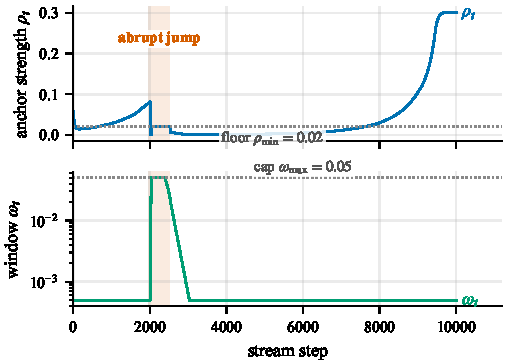
\includegraphics[width=0.55\textwidth]{F4_two_dials}
\caption{Both estimators self-calibrate on a stream with an abrupt jump ($D = 128$, decay-3, seed 0): the anchor strength $\rho_t$ falls on conflict (Proposition~\ref{prop:conflict}) and the window $\omega_t$ opens on drift (Theorem~\ref{thm:window}), both recovering; dotted lines mark the $\rho$ floor and the $\omega$ cap.}
\label{fig:cliffdials}
\end{figure}

\begin{table}[htbp]
\centering
\small
\caption{Stress suite (4 configurations $\times$ 5 seeds): mean and worst overall MSE, one fixed setting per method. The suite is deliberately outside the main grid's operating envelope (loss of persistent excitation, oscillating drift, a stationary control, heavy-tailed rotation noise); the true-noise Kalman is an oracle comparator, and the covariance-form recursion diverges in all 20 runs.}
\label{tab:stress}
\begin{tabular}{lcc}
\toprule
method & mean MSE & worst MSE \\
\midrule
Kalman, true noise ($q = 10^{-4}$) & $1.29$ & $6.26$ \\
SPAR-EG$^+$ & $1.60$ & $7.83$ \\
SPAR-EG & $1.60$ & $7.77$ \\
leaky RLS, information form ($\lambda = 0.99$) & $1.61$ & $7.70$ \\
SPAR-Pull & $1.66$ & $8.10$ \\
SGD ($\mathrm{lr} = 0.01$) & $2.07$ & $10.03$ \\
Adam ($\mathrm{lr} = 0.01$) & $2.82$ & $13.32$ \\
WiSE-FT ($\alpha = 1$) & $3.62$ & $17.39$ \\
anchor-free solve & $4.08$ & $19.70$ \\
frozen warm solution & $5.91$ & $28.83$ \\
leaky RLS, covariance form ($\lambda = 0.99$) & \multicolumn{2}{c}{diverged (20/20)} \\
\bottomrule
\end{tabular}
\end{table}

On the stress suite SPAR-EG$^+$ is the best oracle-free method in mean MSE ($1.60$), $23\%$ below SGD and $43\%$ below Adam; the true-noise Kalman leads it by $23\%$, consistent with the suite residing outside the self-calibration's design envelope (short streams and stationary controls favor fixed shrinkage, Section~\ref{sec:limitations}).

\begin{table}[htbp]
\centering
\scriptsize
\setlength{\tabcolsep}{3pt}
\caption{Marginal mean MSE over the 27 main configurations (each row averages 9 configurations $\times$ 5 seeds), addressing the aggregate-only view of Table~\ref{tab:grid}. The two SPAR methods agree within $0.03$ on every slice; the Kalman and VFF leaders are prior-independent and lose the covariance-rotation slice. The \texttt{abrupt} and \texttt{both} rows coincide to three decimals because both streams carry the same abrupt target jump, and the added covariance rotation shifts the drift-axis mean by less than $10^{-3}$.}
\label{tab:marginal}
\begin{tabular}{llccccc}
\toprule
axis & value & SPAR-Pull & SPAR-EG$^+$ & KF-slow & VFF & leaky-info \\
\midrule
spectrum & isotropic & $0.673$ & $0.644$ & $0.507$ & $0.562$ & $0.636$ \\
 & decay-3 & $0.114$ & $0.115$ & $0.065$ & $0.120$ & $0.257$ \\
 & rank-deficient & $0.131$ & $0.132$ & $0.071$ & $0.119$ & $0.134$ \\
\midrule
drift & abrupt & $0.454$ & $0.440$ & $0.310$ & $0.387$ & $0.487$ \\
 & covariance rotation & $0.011$ & $0.011$ & $0.023$ & $0.027$ & $0.054$ \\
 & both & $0.454$ & $0.440$ & $0.310$ & $0.387$ & $0.487$ \\
\midrule
prior & oracle & $0.301$ & $0.294$ & $0.215$ & $0.267$ & $0.342$ \\
 & warm & $0.305$ & $0.295$ & $0.215$ & $0.267$ & $0.342$ \\
 & adversarial & $0.313$ & $0.303$ & $0.215$ & $0.267$ & $0.342$ \\
\bottomrule
\end{tabular}
\end{table}

\textbf{Methods.}
Each configuration runs the baseline families below in a common streaming protocol, plus the slow-horizon estimated-$R$ Kalman, the variable forgetting factor baselines, the two OGD variants (scalar segment and $D$-dimensional profile), SPAR-EG$^+$, and the causally-tuned Kalman filters appended post hoc. The families are the frozen warm solution, an anchor-free solve, leaky RLS at $\lambda \in \{0.999, 0.997, 0.995, 0.99\}$ in both the covariance-form recursion and the batch information-form solve, directional forgetting at the matched grid $\lambda_f \in \{0.999, 0.997, 0.995, 0.99, 0.98, 0.95, 0.90\}$, AROW at $r \in \{0.01, 0.05, 0.1, 0.3, 0.5\}$, random-walk Kalman filters at $q \in \{10^{-6}, 10^{-5}, 10^{-4}\}$ with the true noise level plus the estimated-$R$ variants at both horizons, SGD at $\mathrm{lr} \in \{0.003, 0.01\}$ and Adam at $\mathrm{lr} \in \{0.0003, 0.001, 0.003, 0.01\}$, variable forgetting factor RLS at two floors under both the single-step and the nominal-length calibrations, and the WiSE-FT $\alpha$-envelope (11 values). The SPAR methods are scalar, diagonal, two-estimator, and expert-simplex.
Sweeps are reported per value; the table reports each family's best setting under both the per-configuration rule (oracle-tuned baselines, the conservative treatment) and the global single-setting rule, and SPAR methods use the same configuration in every cell.

\textbf{Baseline verification.}
Before any comparison, the \texttt{verify} step of the pipeline checks the implementation identities numerically: directional forgetting at $\lambda_f = 1$ coincides with RLS, the Kalman filter at $q = 0, R = 1$ coincides with RLS, and the WiSE-FT endpoints coincide with the frozen and fully adapted solves (maximum absolute deviation of order $10^{-15}$).
The same step checks the algebraic identities of Section~\ref{sec:theory} symbolically (sympy), and the step exits nonzero on any failure.

\textbf{Estimated-noise Kalman.}
The grid includes two estimated-$R$ Kalman filters.
The fast variant updates $R$ with a 100-step moving average of squared residuals; a fast horizon attributes part of the drift-induced residual to measurement noise, which suppresses the filter's gain precisely when adaptation is needed, and it collapses to $1.09/5.36$.
The slow variant uses a $20{,}000$-step horizon (matching the SPAR noise baseline) and attains $0.215/0.93$ (best single $q = 10^{-4}$), within $5.4\%$ of the true-noise filter ($0.204/0.86$) and ahead of SPAR-Pull overall ($0.306/1.22$), though SPAR-Pull leads it on all nine covariance-rotation configurations ($0.011$ vs.\ $0.023$ per configuration mean).
Together, the two rows show that the apparent gap was caused by the estimation horizon, not by access to the true noise level.

\textbf{Rank-deficiency note.}
The prediction-unit estimator never forms $\mathrm{tr}(\bar A^{-1})$: $d_{\mathrm{act}}$ counts only the eigenvalues of $\bar A$ above the $10^{-8}$ numerical ridge, so dead directions contribute neither variance nor conflict and feature rescaling leaves $\rho$ invariant (Appendix~\ref{app:hyper}).
The floor/cap pair bounds the resulting strength in all $135$ main-grid and $20$ stress-suite runs; no SPAR method diverged on any spectrum.

\textbf{Divergence boundary.}
The leaky covariance-form recursion is one tuning step from failure on this grid: $\lambda = 0.997$ attains $0.555$ mean MSE, $\lambda = 0.995$ attains $182$ (worst $3{,}878$), and $\lambda = 0.99$ attains $1.2 \times 10^6$, diverging in $135/135$ main-grid and $20/20$ stress-suite runs (nominal window $100 < D = 128$); Figure~\ref{fig:cliffapp} plots the sweep.
The batch information-form solve of the same objective is stable at every $\lambda$ ($0.34$ mean at $\lambda = 0.99$), which locates the explosion in the covariance recursion rather than the objective; the family's $\lambda$-sensitivity remains (its best stable window is $1.1\times$ SPAR's).

\begin{figure}[htbp]
\centering
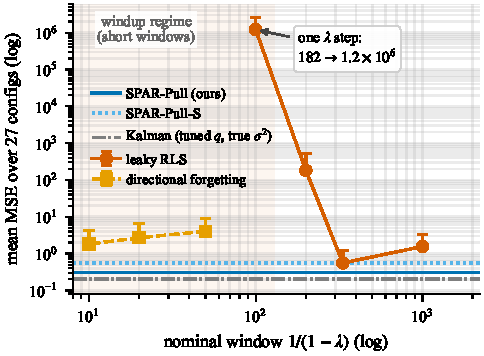
\includegraphics[width=3.1in]{F3_lambda_cliff}
\caption{Mean MSE over 27 configurations versus nominal window $1/(1-\lambda)$ (log--log; $+1$ s.d.\ whiskers). Leaky RLS degrades in one $\lambda$ step ($182 \to 1.2 \times 10^6$ at window $200 \to 100$); shading marks the windup regime ($\mathrm{window} < D = 128$); directional forgetting is divergence-free but $3.3\times$ worse at its best; SPAR-Pull and the scalar SPAR method use one fixed configuration everywhere.}
\label{fig:cliffapp}
\end{figure}
A diagnostic log of the forgetting factor (\texttt{diagnostics.py} \texttt{--diag vff}, \texttt{results/vff\_diag.csv}) confirms the degeneracy: under the reference calibration $\xi = \sigma_0^2$ the factor remains pinned at its floor on $96\%$ of steps on both stationary and drifting streams (mean $\lambda = 0.990$ at floor $0.99$), and a recursive-scale variant of the rule (a Fortescue-style running $\xi$) still pins at the floor ($92\%$ of steps, overall MSE within $2\%$ of the best fixed-$\lambda$ method).
Residual-driven forgetting degenerates to fixed-$\lambda$ leaky RLS whenever $\xi$ tracks the residual scale, a saturation documented in the variable-forgetting-factor literature \citep{paleologu2008}.
The covariance-form VFF inherits the same calibration sensitivity: the single-step normalization $\xi = \sigma_0^2$ drives the factor below $D$ and it diverges identically, while the nominal-length normalization $\xi = N_0\sigma_0^2$ of the original formulation keeps the nominal window near $N_0$ and is stable (best single setting $N_0 = 100$: $0.267/0.98$; the single-step calibration diverges in all 135 runs), the horizon choice $N_0$ playing the role of the fixed window that SPAR's window estimator sets online.
The first-order family terminates at its own boundary: at $\mathrm{lr} = 0.02$, one grid step above the swept maximum, SGD diverges on 45 of 135 runs, and at $\mathrm{lr} = 0.05$ the recursion overflows outright (\texttt{diagnostics.py} \texttt{--diag sgd}); the reported grid $\{0.003, 0.01\}$ sits at the stable frontier of the constant-step family.

\subsection{Windup mechanism}
The covariance-form divergence obeys one law with two channels: whatever the rank-one downdate cannot see inflates by $(1{-}\omega)^{-1}$ per step, growth like $e^{\omega T}$ in the stream length.
On full-rank spectra the unseen component is roundoff: the exponentially weighted covariance matrix is a positive combination of $T \gg D$ outer products, full-rank almost surely at every window, with limiting spectral support bounded away from zero (the lower edge obeys $\lambda - \ln\lambda = 1 + c$, positive for all $c$); the iterated inverse $P \leftarrow (P - kk^\top)/(1{-}\omega)$ instead accumulates antisymmetric roundoff error, and a one-line symmetrization $P \leftarrow \tfrac12(P + P^\top)$ isolates this channel (\texttt{diagnostics.py} \texttt{--diag windup}; 2 representative configurations $\times$ 2 seeds per row):

\begin{table}[h]
\centering
\small
\caption{Mean MSE of the covariance-form leaky recursion on full-rank spectra, with and without per-step symmetrization of the iterated inverse.
At the longest window both variants agree to machine precision; at short windows the unsymmetrized recursion diverges at both dimensions while the symmetrized variant remains stable at every window tested.}
\label{tab:windup-mech}
\begin{tabular}{lccc}
\toprule
$\lambda$ ($1/(1-\lambda)$) & $D$ & standard recursion & symmetrized \\
\midrule
$0.997$ ($333$) & 128 & $1.15$ & $1.15$ \\
$0.995$ ($200$) & 128 & $25.1$ & $0.80$ \\
$0.99$ ($100$) & 128 & $2.8 \times 10^{4}$ & $0.61$ \\
$0.99$ ($100$) & 512 & $7.0 \times 10^{4}$ & $10.4$ \\
\bottomrule
\end{tabular}
\end{table}

On rank-deficient spectra the second channel is deterministic: the dead directions receive no data, so nothing downdates the corresponding block of $P$ and it inflates by $(1{-}\omega)^{-t}$ in exact arithmetic, symmetrized or not.
The appended symmetrized grid method confirms the split (\texttt{append\_arms.py}, \texttt{rls\_sym} rows of \texttt{results/factorial\_extras.csv}): stable on all 90 full-rank runs ($0.13$ mean on the ill-conditioned spectrum, $0.60$ isotropic, at $\lambda = 0.99$) and divergent on 42 of 45 rank-deficient runs ($45$ of $45$ at $\lambda = 0.97$).
The anchored information form is immune to both channels by construction---it never iterates an inverse---and Proposition~\ref{prop:windup} bounds its conditioning for any data and any window.
The single-step VFF calibration enters the same regime through its floor (windows $20$--$100$ at $\lambda_{\min} \in \{0.95, 0.99\}$); the nominal-length calibration keeps windows near $N_0$, above the amplification threshold at every setting tested.

\subsection{False-escalation calibration}
The calibration experiment of Proposition~\ref{prop:falsealarm} runs 300 stationary streams per spectrum through the SPAR estimator with a fixed, calibrated model, records the two-scale residual statistic $z_t = (\widehat\sigma^2_{\mathrm{fast}} - \widehat\sigma^2_{\mathrm{slow}})/\sigma^2$, and measures the fraction of streams whose maximum exceeds the windowed threshold $\tau(\delta) = \sqrt{2\log(T/\delta)/m}$ at the fast horizon $m = 100$.
The measured rate is $0.003$ on isotropic spectra at nominal $\delta = 0.10$ and $0.040$ on ill-conditioned spectra at nominal $\delta = 0.05$, at or below the nominal level; at $\delta = 0.01$ the ill-conditioned rate is $0.033$---the exceedance is predicted by the sub-exponential threshold's linear branch: at $\delta = 0.01$ and $m = 100$, the linear term $2 b_z \log(T/\delta)/(cm)$ dominates the quadratic branch, so the Gaussian-form threshold $\sqrt{2\log(T/\delta)/m}$ used in the calibration experiment is provably too low by the $b_z$-scaling of the moving-average's heavy tail, and the measured $0.033$ exceeds the nominal $0.01$ accordingly.

\subsection{Ablation and sensitivity}
The ablation (\texttt{scripts/revision\_runs.py --suite ablation}) runs the prediction-unit method and its ablations on 4 representative configurations (abrupt and oscillating drifts, adversarial prior, ill-conditioned spectrum) $\times$ 5 seeds.
Removing the window estimator (fixed $\omega$) costs $+189\%$ overall MSE, removing the two-scale residual detector $+190\%$, and removing the pull-identity refresh $+189\%$; setting $\gamma = 0.5$ costs $+560\%$, which measures the $\gamma = 1$ principle of Appendix~\ref{app:proof-dominance}.
Freezing the strength estimator to its warm-up value \emph{lowers} overall MSE by $2.2\%$ on these configurations, and removing the variance-floor subtraction costs $+1.7\%$ under the nominal cap, with the undebiased estimator pinning the window at its cap as Theorem~\ref{thm:window} predicts.
The three-way dissociation in Table~\ref{tab:ablation} localizes the prior-immunity mechanism: freezing the spectral anchor refresh costs $2.2\times$ on the warm-prior configurations and $7.4\times$ on the adversarial ones (adversarial early MSE $47.0$ vs.\ $16.4$), whereas freezing $\rho$ leaves both within $2.6\%$.
Prior immunity is therefore carried by the refresh, and the strength estimator's role is the drift-onset conflict response measured in Appendix Figure~\ref{fig:cliffdials}---it matters only when the warm-up prior scale is unknown, where it guards against an oversized anchor.
An alternating-trust diagnostic probes the strength estimator's average-case value directly (\texttt{diagnostics.py} \texttt{--diag alt\_trust}: the target switches every 500 steps between a noisy revisit of the anchor and a drifted target, two spectra, 5 seeds): the adaptive rule attains $6.79$ overall MSE against $6.64$--$7.00$ for pinned strengths spanning three orders of magnitude ($10^{-3}$ to $1$)---a $\pm 3\%$ spread, because the anchor \emph{refresh}, not the strength estimator, carries the phase-to-phase adaptation.

\begin{table}[h]
\centering
\footnotesize
\caption{Component dissociation on the 4-configuration ablation suite (mean $\pm$ s.d.\ over 20 runs per cell; early MSE is the first 500 post-jump steps). Freezing the anchor refresh is the only variant that loses prior immunity; freezing the strength estimator is indistinguishable from the full method.}
\label{tab:ablation}
\begin{tabular}{lccc}
\toprule
variant & warm overall & adversarial overall & adversarial early \\
\midrule
full & $2.26 \pm 3.28$ & $1.04 \pm 0.21$ & $16.4 \pm 3.3$ \\
fixed $\rho$ (refresh on) & $2.20 \pm 3.16$ & $1.05 \pm 0.21$ & $16.5 \pm 3.3$ \\
frozen anchor (no refresh) & $4.98 \pm 6.49$ & $7.69 \pm 1.62$ & $47.0 \pm 10.2$ \\
no variance floor & $2.30 \pm 3.33$ & $1.06 \pm 0.21$ & $16.7 \pm 3.3$ \\
\bottomrule
\end{tabular}
\end{table}

The dichotomy is exact: the naive estimator $\hat\nu^2_{\mathrm{naive}}(\omega) = (\widehat\E[r_t^2] - \hat\sigma^2)\omega^2$ yields a cubed estimator $(T_{\mathrm{naive}}(\omega))^3 = (\omega^*)^3 + 4\omega^3/(2-\omega) > 2\omega^3$ for every $\omega \in (0,2)$, so the cubed trajectory doubles each iteration and reaches the cap in $O(\log)$ steps even at zero drift (\texttt{naive\_dial\_no\_fixed\_point}), while the variance-floor-subtracted estimator gives the exact affine contraction $u_{m+1} = (1-\eta_\nu)u_m + \eta_\nu(\omega^*)^3 \to (\omega^*)^3$ from any initialization (\texttt{debiased\_dial\_contraction})---both formalized in \texttt{Core.lean}.
Replacing $\mathrm{tr}(\bar A^{-1})$ with the ridge-damped trace $\mathrm{tr}((\bar A + \rho I)^{-1})$ on the rank-deficient configurations (\texttt{append\_damped\_trace.py}, \texttt{results/damped\_trace.csv}) yields identical error ($0.100$ vs.\ $0.100$ overall): the residual-detector and floor branches govern the estimator where the trace saturates, and the damped variant is the numerically preferred implementation on ill-conditioned spectra.
The sensitivity variants (legacy parameter-unit method, \texttt{results/ablation\_spar\_kf.csv}; the control constants are shared with the prediction-unit method) scale the residual horizons ($\pm$), the refresh cadence ($10 \to 50$), the reference-anchor cadence, and the window cap ($0.05 \to 0.02$ and $0.10$): six of the seven variants change overall MSE by at most $\pm 10\%$, and the largest change is the window cap $\omega_{\max} = 0.02$ at $+16\%$.

\subsection{The conflict estimator at drift onset}
\label{app:transient}

Table~\ref{tab:transient} pins the strength at $\rho \in \{0.01, 0.1, 1\}$ with the refresh on and compares it with the adaptive estimator on the abrupt-jump stream with the decay-3 spectrum (5 seeds; \texttt{scripts/transient\_test.py}, \texttt{results/transient\_test.csv}).
At cadence $k = 10$ the adaptive estimator is $1\%$ below the best fixed strength and the large-anchor policy costs $87\%$ more; at $k = 50$ it is within $5\%$ of the best fixed strength while the large-anchor policy costs $2.8\times$.
The penalty is pre-drift, not post-jump: $\rho = 1$ multiplies the pre-drift MSE by $4.2$ relative to the small fixed anchor ($0.049$ vs.\ $0.012$ at $k = 10$) because the anchor holds a warm prior that the decaying spectrum no longer supports, whereas the $50$-step post-jump window is dominated by the jump magnitude and is flat across the adaptive and small-anchor policies---if anything slightly better for the large anchor ($7.7$ vs.\ $9.5$).
On the isotropic spectrum, where a scalar strength has no structural effect, every policy has the same pre-drift MSE ($0.0104$) and differs only through the post-jump term.
We therefore read $\rho_t$ as a guard against a badly oversized anchor---the failure mode a good warm prior invites---not as a post-jump accelerator.

\begin{table}[!htbp]
\centering
\footnotesize
\caption{Transient strength sweep on the abrupt-jump stream, decay-3 spectrum, 5 seeds: pre-drift MSE, MSE over the $50$ steps after the jump, and overall MSE.
The refresh is on in every row; the adaptive row is the paper's method and the others pin $\rho$ for the whole stream.}
\label{tab:transient}
\begin{tabular}{ccccc}
\toprule
$k$ & strength policy & pre-drift MSE & post-jump MSE $[0,50]$ & overall MSE \\
\midrule
10 & adaptive & $0.0136$ & $9.48$ & $\mathbf{0.166}$ \\
10 & fixed $\rho = 0.01$ & $0.0116$ & $9.48$ & $0.168$ \\
10 & fixed $\rho = 0.1$ & $0.0271$ & $9.49$ & $0.195$ \\
10 & fixed $\rho = 1$ & $0.0489$ & $7.72$ & $0.311$ \\
\midrule
50 & adaptive & $0.0197$ & $9.52$ & $0.254$ \\
50 & fixed $\rho = 0.01$ & $0.0146$ & $9.54$ & $\mathbf{0.243}$ \\
50 & fixed $\rho = 0.1$ & $0.0338$ & $9.56$ & $0.308$ \\
50 & fixed $\rho = 1$ & $0.0495$ & $8.52$ & $0.723$ \\
\bottomrule
\end{tabular}
\end{table}

\subsection{Coupling verification}
Theorem~\ref{thm:closedloop}(i)'s condition is measured directly (\texttt{diagnostics.py} \texttt{--diag coupling}, \texttt{results/coupling\_diag.csv}): on the four ablation configurations $\times$ 5 seeds, each estimator is pinned at $\pm 10\%$ of its converged value while the other adapts, and the two sensitivities $L_{\omega\rho}$ (of the cubed window target) and $L_{\rho\omega}$ (of the strength target) are finite-differenced at the empirical coupled fixed point.
The product $L_{\omega\rho} L_{\rho\omega} < 1$ holds in 20 of 20 runs, with maximum $5.7 \times 10^{-3}$---$174$ to $1381$ times below one on the oscillating configuration, the only one with both estimators interior.
On three of the four configurations one estimator saturates at its cap or floor, making the corresponding sensitivity exactly zero---a pinned estimator realizes the triangular specialization of Theorem~\ref{thm:closedloop}(ii), and the large cubed-coordinate slopes recorded at floored windows are boundary artifacts of perturbing a microscopic $u = \omega^3$, multiplied by an exactly-zero factor: the caps act as the coupling control, and the cross-signs at the interior fixed point match the theory ($u^*$ increasing in $\rho$, $\rho^*$ decreasing in $u$).

\subsection{Spectral-risk verification}
Theorem~\ref{thm:rmt}(i)'s closed form was validated at three levels (\texttt{diagnostics.py} \texttt{--diag rmt}).
First, at $45$ fixed operating points (three spectra $\times$ five nominal windows $1/(1-\lambda) \in \{100, \dots, 2000\}$ $\times$ three anchor strengths $\rho \in \{10^{-3}, 10^{-2}, 10^{-1}\}$), the formula matches direct Monte Carlo simulation of the anchored solve ($40$ stationary streams per point, oracle anchor) within $5\%$ relative error on the $30$ full-rank operating points across the entire range, including aspect ratios $\zeta = D\omega$ above one; at the rank-deficient, large-pull corner the error reaches $43\%$, the hard-edge regime we scope as the formula's boundary (\texttt{results/rmt\_grid.csv} records the grid; \texttt{results/rmt\_verify.csv} holds the method-level checks).
Second, at the method's own operating points---the converged estimator pairs $(\omega, \rho)$ measured on stationary streams per spectrum---the formula predicts the method's stationary pre-drift MSE within $2.2\%$ (rank-deficient), $12.7\%$ (ill-conditioned), and $9.8\%$ (isotropic, where the strength estimator sits at its cap), with no fitted parameter.
Third, the closed-form sensitivities of part~(ii) agree with numerical differentiation of the fixed point to $10^{-6}$ relative error.
The pre-drift MSE reported in Section~\ref{sec:experiments} ($1.01$--$1.14 \times \sigma^2$ across spectra) is the segment average including the post-warm-up transient; the formula describes the stationary value at the converged operating pair.

\subsection{Per-step cost}
Table~\ref{tab:app-ops} reports the per-step wall-clock cost of the closed-form methods at $D = 2048$ (fp64 CPU, \texttt{scripts/bench\_ops.py}; run alone for clean timing).
The cached-basis per-direction head is $O(D^2)$ per step with $O(D^3)$ at refreshes; the scalar method solves the anchored system exactly at $O(D^3)$ per step, and its spectral refresh reuses the solve's factorization in $O(D^2)$ (Section~\ref{sec:method-solve}).
The information form deliberately trades the covariance recursion's $O(D^2)$ rank-one update for a factorization that does not wind up on rank-deficient spectra (Proposition~\ref{prop:windup}); where per-step cost dominates, the cached-basis head is the intended path.

\begin{table}[h]
\centering
\footnotesize
\caption{Per-step cost at $D = 2048$ (fp64 CPU).
The cached-basis per-direction head projects each feature into the last refresh's eigenbasis and solves the diagonal system ($O(D^2)$/step, $O(D^3)$ every $k$ refreshes); the scalar method performs a Cholesky factorization plus triangular solves per step ($O(D^3)$), which motivates the per-direction path at large $D$.}
\label{tab:app-ops}
\begin{tabular}{lc}
\toprule
method & ms/step at $D = 2048$ \\
\midrule
leaky RLS & $32.0$ \\
AROW & $31.3$ \\
Kalman & $53.0$ \\
directional forgetting & $56.3$ \\
SPAR-Pull-D (cached basis, $O(D^2)$/step) & $52.6$ \\
SPAR-Pull-S (exact scalar solve, $O(D^3)$/step) & $241$ \\
\bottomrule
\end{tabular}
\end{table}
SPAR-EG and SPAR-EG$^+$ run four batch solves per step (the frozen anchor is the remaining expert in the pool), so their per-step cost is about four times the scalar SPAR-Pull solve timed here; the cached-basis path applies to them as well.

\subsection{Mismatched generators}

\begin{figure}[h]
\centering
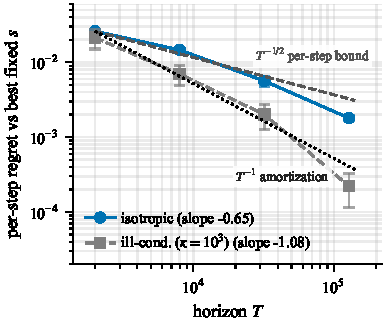
\includegraphics[width=2.9in]{F7_regret_scaling}
\caption{Average per-step regret of the segment (scalar-pull) OGD method versus horizon $T$ (log--log; whiskers: $\pm 1$ s.d.\ over 5 seeds; the drift phase lasts a fixed $1{,}000$ steps at every horizon).
Fitted slopes $-0.65$ (isotropic) and $-1.08$ (ill-conditioned, $\kappa = 10^3$) lie inside the $T^{-1/2}$ per-step rate (dashed) implied by the scalar $O(\sqrt T)$ Zinkevich bound (the $D = 1$ member of the Proposition~\ref{prop:ocowrap}(i) family, formalized as \texttt{ogd\_regret\_segment} in \texttt{Ogd.lean}), with the $T^{-1}$ amortization limit (dotted) as the mechanical floor.}
\label{fig:regret}
\end{figure}

At a fixed horizon, the dimension sweep separates the two gradient variants.
With $T = 9{,}000$, the drift phase held at $1{,}000$ steps, $D \in \{8, 32, 128\}$, and 5 seeds (\texttt{scripts/regret\_dscaling.py}, \texttt{results/regret\_dscaling.csv}), both methods' per-step regret is measured against the best fixed scalar pull (an 11-point segment grid, each comparator method carrying its own refresh trajectory).
The profile method's regret exceeds the segment method's at every operating point, and the gap widens monotonically with $D$---from $0.001$ to $0.078$ on isotropic spectra and from $3 \times 10^{-6}$ to $0.011$ on ill-conditioned spectra---the empirical signature of the $\sqrt{D}$ dimension factor in the Proposition~\ref{prop:ocowrap}(i) bound; on the full grid the same premium appears as the profile method's higher mean MSE ($0.707$ vs.\ $0.585$, Table~\ref{tab:grid}).

\begin{figure}[h]
\centering
\begin{subfigure}[t]{0.48\textwidth}
\centering
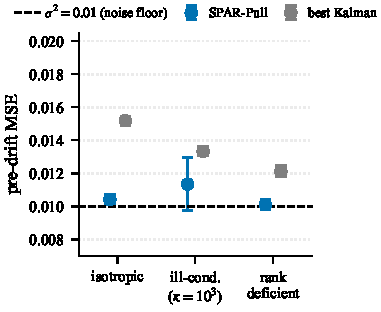
\includegraphics[width=2.55in]{F5_noise_floor}
\caption{}
\label{fig:floor}
\end{subfigure}\hfill
\begin{subfigure}[t]{0.48\textwidth}
\centering
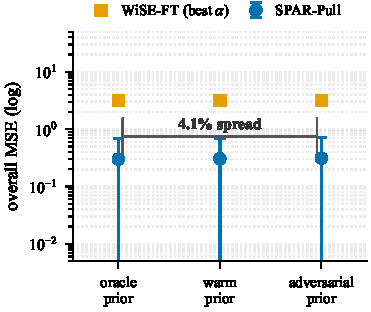
\includegraphics[width=2.55in]{F6_prior_immunity}
\caption{}
\label{fig:prior}
\end{subfigure}
\caption{(a) Pre-drift MSE remains at the irreducible floor $\sigma^2 = 0.01$ across all three spectra (dots show 5-seed means $\pm 1$ s.d.\ against the best tuned-$q$ Kalman with true $\sigma^2$), illustrating Proposition~\ref{prop:conflict} at the optimum.
(b) Overall MSE (log scale) across oracle, warm, and adversarial priors (means over all runs).
While the WiSE-FT best-$\alpha$ envelope sits near $3.2$ under every prior, SPAR-Pull varies by only $4.1\%$ across all three priors (bracket): Proposition~\ref{prop:minimax}.}
\label{fig:floorprior}
\end{figure}

Three generators violate the linear-Gaussian, constant-rate model class: nonlinear targets ($y = \tanh(x^\top w^*) + \varepsilon$; the linear head is misspecified), covariate shift (the feature scale doubles mid-stream), and a noise-regime change ($\sigma^2$ rising from $0.01$ to $0.05$ at $t_1$, with no target drift).
On nonlinear targets (four configurations: decay3 and isotropic spectra under abrupt, gradual, and stationary drifts; 5 seeds each) SPAR-EG$^+$ attains $0.221$ overall MSE, SPAR-EG $0.222$, the best single leaky window ($\lambda = 0.997$) $0.232$, and SPAR-Pull $0.273$: the mixture shifts weight toward the expert that tolerates the nonlinearity.
Under covariate shift the Kalman family leads ($0.268$ with the true noise, $0.284$ with the slow estimated $R$), while SPAR-EG$^+$ and SPAR-Pull lead the anchored and leaky methods ($0.490$ and $0.492$), ahead of the batch-solved leaky method ($0.550$), SPAR-EG ($0.566$), and the best single leaky window ($0.627$), the two-scale residual detector catching the scale change.
Under the noise-regime change (two configurations, decay3 and isotropic spectra, 5 seeds each) the fast-horizon estimated-$R$ Kalman attains $0.069$--$0.098$, its $20{,}000$-step-horizon sibling $0.084$--$0.110$, and the true-noise filter $0.096$--$0.114$ (its fixed $R$ is wrong after the change), while the SPAR-EG mixture attains $0.047$--$0.087$ and SPAR-EG$^+$ $0.047$--$0.053$; SPAR-Pull holds $0.052$ on the decay3 spectrum but lags at $0.080$ on the isotropic spectrum, where its slow noise baseline tracks the pre-change level.
No SPAR method diverged under any mismatch, while the $\lambda = 0.995$ leaky method diverged on nonlinear targets (two of five seeds on the decay3 spectrum under abrupt drift) and degraded under the noise change ($9.1$ and $9.4\times 10^3$ overall MSE).

\subsection{A real high-dimensional stream: hourly electricity load}
\label{app:realstream}

The factorial grid is synthetic, so we also run the grid-default configuration, unchanged, on a real stream: the public hourly electricity-load panel (321 clients, $26{,}304$ hours) \citep{trindade2015electricity,lai2018lstd}.
Features at hour $t$ are the standardized log-loads of all 321 clients plus an intercept and hour-of-day sine/cosine ($D = 324$); the target is the log-load of one held-out client (the 25th-percentile client by mean load) one hour ahead, centered on its warm-up mean.
The warm-up is $2{,}000$ hours and the evaluation horizon $6{,}000$ hours, so $T > 5{,}000$ and $D > 128$ as required.
The stream is not stationary: load carries daily and weekly cycles and a seasonal trend, and the target series moves with them.

Both SPAR methods use the grid defaults of Table~\ref{tab:hyper} unchanged: window range $[5 \times 10^{-4}, 0.05]$, refresh cadence 10, residual horizon 30, and the drift-active floor $0.02$.
The baselines are swept on the same stream and reported at their best setting, which is oracle tuning in their favour: leaky RLS over $\lambda \in \{0.99, 0.995, 0.999\}$ and the slow estimated-$R$ Kalman over $q \in \{10^{-4}, 10^{-5}\}$.

\begin{table}[!htbp]
\centering
\footnotesize
\setlength{\tabcolsep}{5pt}
\caption{Real stream (hourly electricity load, $D = 324$, $T = 6{,}000$ evaluation hours, 25th-percentile held-out client): MSE of the next-hour log-load over the full horizon and over the final $2{,}000$ hours.
SPAR methods use the factorial-grid defaults with no stream-specific tuning; baseline hyperparameters are swept on the same stream and reported at their best.}
\label{tab:electricity}
\begin{tabular}{lcc}
\toprule
method & full horizon & final $2{,}000$ h \\
\midrule
leaky RLS, information form ($\lambda = 0.999$) & $\mathbf{0.0209}$ & $\mathbf{0.0134}$ \\
leaky RLS ($\lambda = 0.995$) & $0.0219$ & $0.0160$ \\
leaky RLS ($\lambda = 0.99$) & $0.0228$ & $0.0174$ \\
Kalman, slow estimated $R$ ($q = 10^{-5}$) & $0.0660$ & $0.0170$ \\
Kalman, slow estimated $R$ ($q = 10^{-4}$) & $0.3054$ & $0.0183$ \\
\midrule
SPAR-EG$^+$ (grid defaults) & $0.0212$ & $0.0143$ \\
SPAR-Pull (grid defaults) & $0.0232$ & $0.0154$ \\
\bottomrule
\end{tabular}
\end{table}

\begin{table}[!htbp]
\centering
\footnotesize
\setlength{\tabcolsep}{5pt}
\caption{Real stream, held-out client sweep: MSE of the next-hour log-load over the full $6{,}000$-hour horizon for the 25th-, 50th-, and 75th-percentile clients by mean load.
The oracle column is the best of the three leaky windows ($\lambda \in \{0.99, 0.995, 0.999\}$) chosen \emph{per client} ($\lambda = 0.999, 0.995, 0.995$ at the 25th, 50th, 75th percentiles)---tuning in the baseline's favour---while the SPAR methods use the grid defaults with no stream-specific tuning.
Bold marks the best entry in each row.}
\label{tab:electricity-clients}
\begin{tabular}{lccc}
\toprule
held-out client & best oracle leaky & SPAR-EG$^+$ & SPAR-Pull \\
\midrule
25th percentile & $\mathbf{0.0209}$ & $0.0212$ & $0.0232$ \\
50th percentile & $0.0086$ & $\mathbf{0.0083}$ & $0.0090$ \\
75th percentile & $\mathbf{0.0112}$ & $0.0113$ & $0.0130$ \\
\midrule
three-client mean & $\mathbf{0.0136}$ & $\mathbf{0.0136}$ & $0.0151$ \\
\bottomrule
\end{tabular}
\end{table}

Across the sweep, SPAR-EG$^+$ lands within $1.2\%$ of the per-client oracle window and $4.3\%$ below it at the 50th percentile, and it matches the oracle on the three-client mean ($0.0136$ both); SPAR-Pull is $4.2$--$16.5\%$ above the oracle.
The ordering of the closed-form methods is stable across the three clients, so the untuned transfer is not specific to a single reported percentile.

Three observations.
First, the untuned SPAR-EG$^+$ lands $1.1\%$ above the best oracle-tuned leaky window over the full horizon and $6.3\%$ above it on the final $2{,}000$ hours, while SPAR-Pull is $10.7\%$ and $14.7\%$ above; a smooth seasonal stream has a long and nearly constant optimal window, which is exactly the regime in which a fixed long window is close to optimal and adaptation has little to recover.
Second, the slow estimated-$R$ Kalman is far worse over the full horizon ($0.051$ and $0.257$) and still $26\%$ above the leaky baseline on the final $2{,}000$ hours, i.e.\ its early noise estimates are poor and it only recovers late.
Third, no method diverges and the ordering of the closed-form methods is stable across the horizon, so the control law transfers to a real $D = 324$ stream without retuning.

\section{BCI IV details}
\label{app:eeg}
\setcounter{figure}{0}\setcounter{table}{0}

\textbf{Datasets and protocol.}
BCI Competition IV 2a \citep{brunner2008bci2a} and 2b \citep{leeb2008bci2b}, nine subjects each, loaded from the npz cache described in Appendix~\ref{app:repro}.
Cross-session protocol: each method fits on the training session and streams the evaluation session (288 trials on 2a, 320 on 2b) predict-then-update.
All online methods use supervised adaptation: the label of trial $t$ enters after its prediction, so every prediction is prequential.
Labels are one-hot $Y_t \in \{0,1\}^K$; the streaming head maintains a $D \times K$ coefficient matrix and the scalar residual driving both estimators is $r_t^2 = \|Y_t - \widehat Y_t\|_2^2/K$.
The metric is balanced accuracy; with $n = 9$ subjects per dataset we report paired tests and effect sizes, not significance alone.

\begin{table}[h]
\centering
\scriptsize
\setlength{\tabcolsep}{2.5pt}
\renewcommand{\arraystretch}{0.86}
\caption{BCI IV cross-session, balanced accuracy (mean $\pm$ s.d.\ over 9 subjects per dataset).
Supervised online protocol for adaptive methods; classical methods are static. $^{\mathrm{T}}$Session-level Euclidean alignment from the unlabeled evaluation session (transductive); the online-EA row is strictly causal.
Highest value per column in bold.}
\label{tab:eeg}
\begin{tabular}{lcc}
\toprule
method & BCI IV 2a & BCI IV 2b \\
\midrule
\multicolumn{3}{l}{\emph{classical (canonical implementations)}}\\
MDM (pyriemann) & $0.566 \pm 0.160$ & $0.728 \pm 0.148$ \\
FgMDM (pyriemann) & $0.641 \pm 0.171$ & $0.755 \pm 0.149$ \\
LDA (raw features) & $0.480 \pm 0.069$ & $0.651 \pm 0.107$ \\
LDA (raw) + session EA$^{\mathrm{T}}$ & $0.563 \pm 0.076$ & $0.677 \pm 0.133$ \\
CSP-LDA (mne) & $0.607 \pm 0.151$ & $0.749 \pm 0.141$ \\
tangent cov + LDA & $0.637 \pm 0.165$ & $0.752 \pm 0.147$ \\
cov-LDA, offline session-EA$^{\mathrm{T}}$ & $0.664 \pm 0.173$ & $0.728 \pm 0.159$ \\
\midrule
\multicolumn{3}{l}{\emph{ours (closed-form streaming, predict-then-update)}}\\
CSP + SPAR-Pull & $0.627 \pm 0.159$ & $0.770 \pm 0.142$ \\
tangent cov + SPAR-Pull & $0.527 \pm 0.151$ & $0.772 \pm 0.129$ \\
hybrid + SPAR-Pull$^{\mathrm{T}}$ & $0.597 \pm 0.137$ & $0.808 \pm 0.104$ \\
hybrid + SPAR-Pull, grid defaults$^{\mathrm{T}}$ & $0.579 \pm 0.137$ & $0.801 \pm 0.101$ \\
online-EA + hybrid + SPAR-Pull & $0.596 \pm 0.134$ & $0.801 \pm 0.105$ \\
hybrid + AAL head ($\gamma{=}1$, fixed anchoring)$^{\mathrm{T}}$ & $0.608 \pm 0.139$ & $0.799 \pm 0.107$ \\
hybrid + leaky head$^{\mathrm{T}}$ & $0.554 \pm 0.123$ & $0.812 \pm 0.108$ \\
hybrid + SPAR-EG$^{\mathrm{T}}$ & $0.580 \pm 0.130$ & $\mathbf{0.816 \pm 0.102}$ \\
hybrid + SPAR-EG$^{+\,{\mathrm{T}}}$ & $0.586 \pm 0.141$ & $0.813 \pm 0.107$ \\
\midrule
\multicolumn{3}{l}{\emph{backprop references}}\\
EEGNet-lite (train-split tuned, zero-shot) & $0.556 \pm 0.080$ & $0.776 \pm 0.129$ \\
WiSE-FT on the net (causal, $\alpha$-envelope) & $0.591 \pm 0.079$ & $0.811 \pm 0.115$ \\
\midrule
post-hoc ensemble (cov-LDA + hybrid warm fit)$^{\mathrm{T}}$ & $\mathbf{0.668 \pm 0.175}$ & $0.771 \pm 0.104$ \\
\bottomrule
\end{tabular}
\end{table}

\textbf{Compute.}
The complete closed-form suite (feature extraction plus all closed-form methods) for all nine 2b subjects runs in $17$ s on the CPU used here ($1.9$ s per subject; \texttt{results/tier1\_rerun\_2b.log}); one EEGNet-lite training configuration ($120$ epochs) trains on the WSL GPU environment, and the full backprop protocol trains three configurations per subject plus the online fine-tuning pass.

\textbf{Feature families.}
Three feature families feed the readouts of Table~\ref{tab:eeg}.
CSP: 6-component CSP (Ledoit--Wolf shrinkage, log output) computed with MNE \citep{gramfort2013mne} on bandpassed epochs (8--30 Hz, 4th-order Butterworth), the classical motor-imagery standard \citep{ramoser2000csp}.
Tangent covariance: per-trial log-Euclidean covariance tangent features (lower triangle) on bandpassed epochs, the feature family of pyriemann's tangent-space methods.
Hybrid: the statistical pipeline (summary statistics, lags $(1, 2, 4, 8)$, FFT bins) concatenated with the tangent-covariance features.
Classical readouts are MDM and FgMDM as implemented in pyriemann \citep{barachant2020pyriemann}, raw-feature LDA with and without session-level Euclidean alignment \citep{he2020ea}, CSP-LDA, tangent-covariance LDA (shrinkage LDA in all cases), and a covariance-LDA method with the same offline alignment.
Streaming readouts are the two-estimator SPAR-Pull head (anchor refresh every 5 trials), the AAL head (fixed $\gamma = 1$ anchoring), and a forgetting-only leaky head, each applied to CSP, tangent-covariance, or hybrid features.

\textbf{Alignment protocol.}
The hybrid methods use session-level Euclidean alignment: per-trial covariance whiteners are computed from each session separately, so the alignment is transductive at the session level (the offline classical methods share this convention).
The strictly online method recomputes its whitener causally from a trailing window of the evaluation stream (40 trials, refreshed every 10) for \emph{both} feature halves: the statistical features and the tangent-covariance features are each whitened with the trailing-window estimate, so no stream feature depends on trials beyond the current one.
All SPAR methods in Table~\ref{tab:eeg} run the same variance-floor-subtracted window inversion as the factorial grid (Theorem~\ref{thm:window}), with the estimator ranges rescaled to the $288$-trial stream (window range $[5\times10^{-3},0.02]$, refresh cadence 5, residual horizon 40, calibration blocks 2).
The \emph{grid defaults} row is the same hybrid head with the factorial-grid window range, refresh cadence, residual horizon, and calibration blocks ($[5\times10^{-4},0.05]$, 10, 30, 10); the gap to the EEG-range row prices those four settings ($0.018$ balanced accuracy on 2a and $0.007$ on 2b).
The reduced range therefore helps, but the ranking of the readouts and the qualitative conclusion (closed-form streaming matches the causal backprop reference) do not depend on it.

\textbf{WiSE-FT protocol measurement.}
Transplanting the original WiSE-FT protocol \citep{wortsman2022wiseft} (fine-tune on the target data, then evaluate on it) into cross-session evaluation is train-on-test.
Measured directly, the offline fine-tuned endpoint reaches accuracy $1.000$ by memorizing the evaluation stream.
The comparison we report is therefore the causal reformulation: the network is fine-tuned online with one SGD step per trial \emph{after} predicting it, trial $t$ is predicted with the interpolation $(1 - \alpha)\,W_{\mathrm{zero}} + \alpha\,W_t$ where $W_t$ is the online model before trial $t$'s label, and the $\alpha$-envelope is swept post-hoc over 11 values with all trajectories causal (the prequential evaluation of Table~\ref{tab:eeg}).

\textbf{Backprop references.}
EEGNet-lite is a small EEGNet variant \citep{lawhern2018eegnet} ($F_1 = 8$, $D = 2$, $F_2 = 16$) trained with Adam.
Its hyperparameters (epochs, learning rate) are selected on an 80/20 split of the training session from the grid $(120, 10^{-3})$, $(300, 10^{-3})$, or $(300, 3 \times 10^{-4})$ with no evaluation-session access, then retrained on the full training session and evaluated zero-shot on the evaluation session.
The WiSE-FT-on-network reference uses this zero-shot model as its frozen endpoint and the causal fine-tuning protocol above.

\section{Hyperparameters and provenance}
\label{app:hyper}
\setcounter{figure}{0}\setcounter{table}{0}

\textbf{Fixed constants and the default control parametrization.}
The complete fixed control parametrization is enumerated in Table~\ref{tab:hyper}: the three headline constants (anchor-refresh cadence 10 steps, fast-EMA residual horizon 30 steps, drift-active anchor-strength floor $\rho \ge 0.02$), the clip ranges of both estimators, the slow-noise-EMA baseline horizon (20{,}000, matched to the estimated-noise Kalman), the reference-anchor EMA horizon (200 steps), the conflict-floor multiplier ($\tfrac12$), the estimator smoothing gains ($\eta_C = 0.15$, $\eta_\nu = 0.2$), and the $10^{-8}$ numerical ridge of the trace and active-dimension computations.
These were fixed once, before the factorial grid, and are shared by every SPAR method on it; all remaining behavior is self-calibrated at runtime by the two online estimators.
The sensitivity analysis of Appendix~\ref{app:protocol} perturbs the headline constants directly.

\begin{table}[htbp]
\centering
\small
\caption{Fixed default control parametrization (grid: $T = 10^4$). The EEG head uses a reduced estimator range and shorter horizons for the short evaluation streams, hand-set once and disclosed here; no per-configuration search was performed for any SPAR method.}
\label{tab:hyper}
\begin{tabular}{lll}
\toprule
parameter & grid default & EEG head \\
\midrule
refresh cadence $k$ & $10$ & $5$ trials \\
fast-EMA horizon $h_f$ & $30$ & $40$ \\
warm-up anchor strength $\rho_0$ & $0.1$ & $0.1$ \\
stationary $\rho$ floor & $10^{-5}$ & $10^{-5}$ \\
drift-active $\rho$ floor & $0.02$ & --- \\
anchor-strength cap $\rho_{\max}$ & $1.0$ & $1.0$ \\
window clip $[\omega_{\min}, \omega_{\max}]$ & $[5\times10^{-4},\ 0.05]$ & $[5\times10^{-3},\ 0.02]$ \\
slow-noise-EMA horizon & $20{,}000$ & $2{,}000$ \\
reference-anchor EMA horizon & $200$ & $30$ \\
conflict-floor multiplier & $\tfrac12$ & $\tfrac12$ \\
smoothing gains $(\eta_C, \eta_\nu)$ & $(0.15,\ 0.2)$ & $(0.2,\ 0.1)$ \\
active-dimension / trace ridge & $10^{-8}$ & $10^{-8}$ \\
\bottomrule
\end{tabular}
\end{table}

\textbf{Estimator floors and caps.}
The window estimator is clipped to $\omega \in [5 \times 10^{-4},\ 0.05]$ on the grid (the floor is no forgetting at the grid's horizon; the cap bounds the forgetting rate), and the anchor-strength estimator enforces the drift-active floor above together with a hard cap.
The EEG head uses a reduced range suited to the short evaluation streams ($\omega \in [5 \times 10^{-3},\ 0.02]$, fast horizon 40, refresh every 5 trials, reference-anchor horizon 30, smoothing gains $(\eta_C,\eta_\nu) = (0.2, 0.1)$) and omits the drift-active floor; these are the only stream-dependent settings in the paper.

\textbf{Conflict estimator branches (prediction units).}
Algorithm~\ref{alg:spar-pull} step (iv) takes the maximum of three branches, all in prediction-risk units $[y^2]$ (the residual EMAs are $\sigma^2_{\mathrm{fast}}$ = fast EMA of $r_t^2$ at horizon $h_f$, $\sigma^2_{\mathrm{slow}}$ = slow EMA at horizon $20{,}000$; $d_{\mathrm{act}}$ is the number of eigenvalues of $\bar A$ above the $10^{-8}$ numerical ridge):
(i) the reference branch $C^\Sigma_{\mathrm{ref}} = (G_{\mathrm{ref}} - \widehat w)^\top \bar A\,(G_{\mathrm{ref}} - \widehat w) - \widehat V^\Sigma$, where $\widehat w$ is the minimum-ridge data solve, $\widehat V^\Sigma = \hat\sigma^2 d_{\mathrm{act}}/n$, and $G_{\mathrm{ref}}$ is the reference anchor (a slow-moving copy of $G$ at the reference cadence, updated every $5k$ steps);
(ii) the residual branch $C^\Sigma_{\mathrm{resid}} = E_t = \max(0, \sigma^2_{\mathrm{fast}} - \sigma^2_{\mathrm{slow}})$;
(iii) the floor $C^\Sigma_{\mathrm{floor}} = \tfrac12\,\hat\sigma^2 d_{\mathrm{act}}/T_w$ (the warm-up prediction variance is an irreducible lower bound on the conflict of a warm-up anchor).
The per-clip strength is $\rho = \mathrm{clip}(\bar\mu\,\widehat V^\Sigma/\widehat C^\Sigma_t,\ \rho_{\min}^{\mathrm{drift}},\ \rho_{\max})$ with the drift-active floor $0.02$ engaged while the window is at least half open ($\omega_t \ge \tfrac12\omega_{\max}$) and the stationary floor $10^{-5}$ otherwise.
Every branch has units $[y^2]$ and $\rho$ has units $[x^2]$; no inverse of $\bar A$ is formed, so the estimator is invariant to feature rescaling and immune to the rank-deficient trace blow-up.
The legacy parameter-unit form (with $\mathrm{tr}(\bar A^{-1})$ and $C_{\mathrm{resid}}=E_t\mathrm{tr}(\bar A^{-1})/(n\bar\mu)$) is reported only as the ablation of Appendix~\ref{app:protocol}.

\textbf{Method identifiers.}
The paper's display names map to frozen artifact identifiers (internal Python/CSV keys) as follows: SPAR-Pull is \texttt{spar\_pull} (its legacy parameter-unit form is \texttt{spar\_kf2}), SPAR-Pull-S is \texttt{spar\_scalar}, SPAR-Pull-D is \texttt{spar\_diag}, SPAR-EG is \texttt{spar\_eg}, SPAR-EG$^+$ is \texttt{spar\_eg\_plus}, the causally-tuned Kalman filters are \texttt{kf\_causal} and \texttt{kf\_est\_causal}/\texttt{kf\_est\_slow\_causal}, the AAL head is \texttt{hybrid-pam\_g1}, leaky RLS is \texttt{leaky[$\lambda$]} in covariance form and \texttt{leaky\_batch} in information form, directional forgetting is \texttt{df[$\lambda_f$]}, AROW is \texttt{arow[$r$]}, the Kalman filters are \texttt{kf[$q$]} (true noise), \texttt{kf\_est} (100-step estimated $R$), and \texttt{kf\_est\_slow} (20{,}000-step estimated $R$), the gradient-descent baselines are \texttt{sgd} and \texttt{adam}, the OGD variants are \texttt{ogd\_profile} (scalar segment) and \texttt{ogd\_profile\_d} (full $D$-dimensional profile), the variable forgetting factor baseline is \texttt{vff[fortescue]} in covariance form and \texttt{vff\_info[fortescue]} in information form, and the WiSE-FT envelope is \texttt{wiseft}.
All renaming in the paper is display-layer only; the CSVs, scripts, and tests key on the artifact identifiers.

\textbf{Seeds.}
All seeds are pinned in the drivers: the factorial grid uses seeds 0--4 per configuration; the ablation, regret scaling, coupling diagnostic, and mismatched-generator studies use seeds 0--4; the false-escalation calibration uses 300 streams (seeds 1000--1299); the estimator-trajectory figure uses seed 0; the EEG evaluation uses subjects 1--9 per dataset (all available subjects); the BP references train with per-subject seeds equal to the subject index.
Seeds are shared across methods at each configuration.

\textbf{Data manifests.}
Synthetic streams are generated from the pinned seeds by the committed generator (\texttt{rls\_baselines.make\_stream\_fac}), so no synthetic data files are needed.
The EEG evaluation reads the committed npz cache (\texttt{data/eeg\_cache/\{2a,2b\}/subject*.npz}), exported from the MNE data directory by \texttt{scripts/export\_eeg\_npz.py}.
Every result table in the paper is machine-printed from a committed CSV under \texttt{results/} (Appendix~\ref{app:repro}).

\section{Reproducibility}
\label{app:repro}
\setcounter{figure}{0}\setcounter{table}{0}

\textbf{One driver.}
A single driver regenerates every figure and every wired result table from the committed caches:
\begin{quote}
\ttfamily
py scripts/run\_all.py --list\ \ list the pipeline steps\\
py scripts/run\_all.py --steps quick\ \ verify+aggregate+figures\\
py scripts/run\_all.py\ \ everything (hours; resumable)
\end{quote}
The quick preset takes about 2 minutes; the full run takes hours and is resumable.
\begin{table}[!htbp]
\centering
\footnotesize
\setlength{\tabcolsep}{4pt}
\caption{One driver, \texttt{scripts/run\_all.py}, runs these stages in order; each is resumable.}
\label{tab:pipeline}
\begin{tabular}{lll}
\toprule
stage & driver & output \\
\midrule
\texttt{verify} & \texttt{verify\_spar\_theorems.py} & symbolic identities \\
\texttt{factorial} & \texttt{synthetic\_factorial.py} & \texttt{factorial\_d\_*.csv} \\
\texttt{sparkf} & SPAR-Pull append & \texttt{factorial\_extras.csv} \\
\texttt{append} & \texttt{append\_arms.py}, \texttt{regen\_spar\_eg\_plus.py}, \texttt{revision\_runs.py --suite grid} & \texttt{factorial\_pu\_refresh.csv} \\
\texttt{aggregate} & \texttt{aggregate\_factorial.py} & Table~\ref{tab:grid} \\
\texttt{ablation} & \texttt{revision\_runs.py --suite ablation} & \texttt{ablation\_spar\_pull.csv} \\
\texttt{falseesc} & 300-stream calibration & \texttt{false\_esc.csv} \\
\texttt{regret} & horizon and dimension scaling & \texttt{regret\_*.csv} \\
\texttt{ops} & wall-clock timing at $D=2048$ & \texttt{ops\_table.csv} \\
\texttt{eeg} & \texttt{bench\_eeg\_tier1.py} & \texttt{eeg\_tier1\_2*.csv} \\
\texttt{bp} & backprop baselines & \texttt{bp\_tta\_2*.csv} \\
\texttt{figures} & \texttt{make\_figures.py} & \texttt{results/figures/} \\
\bottomrule
\end{tabular}
\end{table}

\textbf{Environment.}
Python 3.12 with the committed \texttt{requirements.txt} (jax, numpy, scipy, pandas, scikit-learn, matplotlib, sympy).
Float64 is required for the streaming solves and is enabled by setting \texttt{JAX\_ENABLE\_X64=1} (the drivers set it); a CPU runtime is recommended for the fp64 streams.
The backprop methods run on the WSL GPU virtual environment: \texttt{scripts/run\_bp\_tta\_2a.sh} and \texttt{scripts/run\_bp\_tta\_2b.sh}, with \texttt{BP\_PYTHON} pointing at that environment's interpreter and GPU extras in \texttt{requirements-wsl.txt}.

\textbf{EEG data.}
Raw BCI IV files live under the MNE data directory (\texttt{MNE\_DATA} environment variable or the mne configuration; default \texttt{\~{}/mne\_data}) at the BNCI database path.
The loader prefers the npz cache: run \texttt{scripts/export\_eeg\_npz.py} once to produce \texttt{data/eeg\_cache/\{2a,2b\}/subject*.npz} for all nine subjects per dataset.

\textbf{Electricity data.}
The real stream of Appendix~\ref{app:realstream} reads the public hourly electricity-load panel (321 clients, $26{,}304$ rows, headerless comma-separated) from \texttt{data/ts/electricity.csv} (the loader also accepts the \texttt{.txt} variant); the file is a public download and is not shipped with the artifact.
It regenerates with \texttt{scripts/bench\_stream\_real.py --clients 11,82,171} (\texttt{results/stream\_electricity.csv}); the script accepts any client indices, and the tables report the 25th-, 50th-, and 75th-percentile clients.
The transient strength sweep of Appendix~\ref{app:transient} regenerates with \texttt{scripts/transient\_test.py} (\texttt{results/transient\_test.csv}).
The grid-default BCI row of Table~\ref{tab:eeg} is the \texttt{hybrid-spar\_kf\_grid} column of \texttt{scripts/bench\_eeg\_tier1.py}; on 2a it is also reproduced by the cheaper \texttt{scripts/eeg\_grid\_default\_probe.py}, which saves \texttt{results/eeg\_griddefault\_2a.csv}.

\textbf{Lean.}
The proof artifact builds with the elan-managed Lean 4 toolchain and Mathlib via lake; the full recipe, including the Mathlib cache fetch, is \texttt{theory/lean/build\_ogd.sh} (Appendix~\ref{app:lean}).

\textbf{Artifact layout.}
Every number in the paper is machine-printed into \texttt{results/*.csv} by the drivers above, and every figure is redrawn from those CSVs: the factorial tables (\texttt{factorial\_*}), the ablation (\texttt{ablation\_spar\_pull.csv}), the false-escalation calibration (\texttt{false\_esc.csv}), the regret scaling (\texttt{regret\_scaling.csv}), the cost table (\texttt{ops\_table.csv}), the EEG tables (\texttt{eeg\_tier1\_2*.csv}, \texttt{spar\_eeg\_2*.csv}, \texttt{bp\_tta\_2*.csv}), the estimator trajectory (\texttt{estimator\_trajectory.csv}), the real electricity stream (\texttt{stream\_electricity.csv}), and the transient strength sweep (\texttt{transient\_test.csv}).
The offline session-EA cov-LDA method and the post-hoc ensemble (members: the cov-LDA method and the static hybrid warm fit, identifier \texttt{ens-covlda+hybrid}) regenerate from the \texttt{eeg} step's baseline pass (\texttt{scripts/bench\_eeg.py}, recorded in \texttt{eeg\_2*.csv}); all other rows regenerate from the tier-1 pass.
The Lean material (six files, the build script, and the axiom-listing script) is under \texttt{theory/lean/}.
